\documentclass[11pt]{article}
\usepackage[a4paper,margin=28mm]{geometry}
\usepackage{amsmath,amssymb,amsthm,mathtools,bm}
\usepackage[T1]{fontenc}
\usepackage{lmodern,microtype}
\usepackage{graphicx,tikz,booktabs,array,longtable}
\usetikzlibrary{arrows.meta,positioning,calc}
\usepackage[numbers,sort&compress]{natbib}
\usepackage{xurl}
\usepackage[colorlinks=true,linkcolor=blue,citecolor=blue,urlcolor=blue]{hyperref}
\usepackage{bookmark}
\usepackage{needspace}
\makeatletter
\let\paper@l@part\l@part
\renewcommand*\l@part[2]{\Needspace{5\baselineskip}\paper@l@part{#1}{#2}}
\renewcommand*\l@subsection{\@dottedtocline{2}{1.5em}{3.2em}}
\makeatother
\hypersetup{pdftitle={Row--column symmetry and contraction of coordinate sweeps},pdfauthor={OpenAI}}
\newtheorem{theorem}{Theorem}[section]
\newtheorem{lemma}[theorem]{Lemma}
\newtheorem{proposition}[theorem]{Proposition}
\newtheorem{corollary}[theorem]{Corollary}
\theoremstyle{definition}
\newtheorem{definition}[theorem]{Definition}
\theoremstyle{remark}
\newtheorem{remark}[theorem]{Remark}
\DeclareMathOperator{\Tr}{Tr}
\DeclareMathOperator{\KL}{KL}
\DeclareMathOperator{\Sym}{Sym}
\DeclareMathOperator{\Var}{Var}
\DeclareMathOperator{\Ent}{Ent}
\newcommand{\TV}{\mathrm{TV}}
\newcommand{\HS}{\mathrm{HS}}
\newcommand{\op}{\mathrm{op}}
\newcommand{\E}{\mathbb E}
\newcommand{\PP}{\mathbb P}
\newcommand{\id}{\mathrm{id}}
\newcommand{\eps}{\varepsilon}
\newcommand{\ind}{\mathbf1}
\allowdisplaybreaks[1]
\setlength{\emergencystretch}{2em}
\title{Row--column symmetry and contraction of coordinate sweeps}
\author{OpenAI}
\date{September 26, 2026}
\begin{document}
\maketitle
\begin{abstract}
We prove that the Thorp shuffle on $N=2^d$ labeled cards has full-permutation total-variation mixing time $\Theta(\log N)$ in physical shuffles. An absolute number of coordinate sweeps suffices for the upper bound.
\end{abstract}
\tableofcontents
\section{Introduction}
A coordinate sweep of the Thorp shuffle acts on $N=2^d$ labeled cards.
It scans the $d$ binary coordinates in order and, in each direction,
independently swaps or leaves unchanged the two cards on every parallel edge.
A single card is uniform after a sweep. The full permutation retains
dependence because the cards have used the same switches. We prove that an
absolute number of sweeps suffices to mix the full permutation. Since a
sweep consists of $d$ physical shuffles, this gives the optimal order
$\Theta(\log N)$ in physical shuffle time.

The Thorp shuffle arose in a study of nonrandom shuffling and advantageous play in Faro \cite{Thorp1973}. For $N=2^d$, Morris proved an $O(d^{44})$ bound using evolving sets \cite{Morris2008}; Montenegro and Tetali sharpened the spectral-profile and evolving-set analysis to $O(d^{29})$ \cite[Section~6.4]{MontenegroTetali2006}. Morris then used entropy contraction to obtain $O((\log N)^4)$ mixing for every even deck size \cite{Morris2009}, followed by an $O(d^3)$ bound for dyadic decks \cite{Morris2013}. These estimates concern the full permutation and count individual physical shuffles; one coordinate sweep comprises $d$ such steps.

The $O(d^3)$ full-deck benchmark is also recorded in the November 2025 account of \citet[Section~1]{AlekseevEtAl2025}. Faster bounds for observing a fixed fraction of the cards, such as the $O((\log N)^2)$ bound of \citet{CzumajVocking2014}, concern a different projection of the permutation law. Here we obtain the order $O(d)$ for the full permutation on a dyadic deck, together with quantitative row--column representation estimates. The support bound in Proposition~\ref{ten:support} gives the matching lower order.

To see the geometric issue, split the coordinates into two consecutive
groups. The positions become a rectangular board. The first part of the
sweep acts within rows, and the second within columns; each part consists
of independent smaller sweeps. This suggests an induction on the number
of coordinates. Its obstacle is that the row and column symmetry
decompositions differ, and their projections generally do not commute.
We estimate how much of a vector selected by one decomposition can survive
selection by the other. Three forms of this estimate lead to the same
mixing conclusion while retaining different information about the
representation spaces.

\subsection{The sweep and its moments}
Positions are vectors $x=(x_1,\ldots,x_d)\in\mathbb F_2^d$. A physical
Thorp shuffle sends
\[
 (x_1,u)\longmapsto(u,x_1+\xi_u),
\]
where the $2^{d-1}$ bits $\xi_u$ are independent and fair. Let $q_d$
denote the law of this shuffle. Removing the
deterministic cyclic rotation after each shuffle gives successive matching
updates in the $d$ coordinate directions. After $d$ updates the rotation
is the identity. Thus one coordinate sweep has exactly the law of $d$
physical shuffles.

Permutations map initial positions to final positions, and $gh$ applies
$h$ first. Let $K_d=q_d^{*d}$ denote the law of one sweep. On the complex unitary
irreducible representation $V_\lambda$ of $S_N$, indexed by a partition
$\lambda\vdash N$, put
\[
 D_\lambda=\dim V_\lambda,\qquad
 K_d(\lambda)=\sum_{g\in S_N}K_d(g)\rho_\lambda(g).
\]
A matching layer is an orthogonal projection, so $K_d(\lambda)$ is a
contraction. All traces are ordinary, unnormalized traces, and
$\|A\|_p^p=\operatorname{Tr}|A|^p$. The matrix $K_d(\lambda)$ need not be
normal. On restriction to a subgroup, an irreducible type may occur
several times. We call its representation space the carrier and distinguish
directions within it from the different multiplicity copies.

Our first estimate attaches a positive weight to each Young diagram.
When we pass from the full board to its rows and columns, the difference
between the diagram weights pays for the cost of restoring deleted cells.
The weights still retain a fixed power of representation dimension.
Their construction appears in Section~\ref{ten:weighted:part:60}.

\begin{theorem}[Weighted sweep moments]\label{thm:weighted}
There are positive weights $W_\lambda$, an absolute finite $p_*$, and real
exponents $2\le p_d\le p_*$ such that, for every $d\ge1$ and every
$\lambda\vdash2^d$,
\begin{equation}\label{eq:weighted-main}
 D_\lambda^{3/4}\le W_\lambda\le D_\lambda,
 \qquad W_\lambda\|K_d(\lambda)\|_{p_d}^{p_d}\le1.
\end{equation}
Consequently $\|K_d(\lambda)\|_{\rm op}\le D_\lambda^{-3/(4p_*)}$.
\end{theorem}

The bounded exponent gives a dimension power uniformly over all diagrams
and deck sizes. It also yields a common unweighted moment: for an absolute
$q<\infty$,
\begin{equation}\label{eq:common-unit-moment}
 D_\lambda\|K_d(\lambda)\|_q^q\le1.
\end{equation}
Indeed, at $p=p_d$ the theorem gives
$\|K_d(\lambda)\|_{\rm op}^p\le W_\lambda^{-1}$, and hence
\[
 D_\lambda\|K_d(\lambda)\|_{4p/3}^{4p/3}
 \le D_\lambda W_\lambda^{-4/3}\le1.
\]
Since the matrices are contractions, $q=4p_*/3$ works simultaneously.
The later two routes prove a bound of the form
\eqref{eq:common-unit-moment} directly. Their additional information lies
in the intermediate row--column estimates described below.

We use
$\|\mu-\nu\|_{\rm TV}=\tfrac12\sum_g|\mu(g)-\nu(g)|$.
Let $t_{\rm mix}(d)$ be the least number of physical shuffles for which
the distance from the uniform full-deck law is at most $1/4$, from every
starting deck.
\begin{corollary}[Optimal order of mixing]\label{cor:optimal-mixing}
There is an absolute constant $C$ such that, for every $d\ge1$,
\[
 \left\lceil\frac2N\log_2\frac{3N!}{4}\right\rceil
 \le t_{\rm mix}(d)\le Cd,
 \qquad N=2^d.
\]
In particular $t_{\rm mix}(d)=\Theta(d)$, and its lower bound is
$2d-O(1)$.
\end{corollary}
The upper bound follows from finite-group Plancherel and Cauchy--Schwarz
\cite[Sections~2 and~3]{DiaconisShahshahani1981}, applied to a fixed
number of repeated forward sweeps. The lower bound counts the possible
permutations produced by the random switches. Both deductions are given
in Section~\ref{ten:weighted:part:285}, after the first moment proof.

\subsection{From row--column overlap to a bounded exponent}
The first route begins by choosing a subdiagram $a\subseteq\lambda$
inside an $(h,h)$-hook: no box of $a$ has both row and column index
greater than $h$. If $t=N-|a|$, we let the symmetric group on the
$N-t$ occupied cells of a board act through $V_a$. Hook trimming and the
choice of weights control the cost of making this reduction. The
representation $V_a$ occurs in a tensor space with an $h$-dimensional
even part and an $h$-dimensional odd part. This hook realization is
classical in signed tensor representation theory \cite{BereleRegev1987};
we obtain the form needed here from ordinary Schur--Weyl duality on the
two parts and signed induction.

Theorem~\ref{thm:occupied} bounds overlap on every occupied-cell pattern,
summing over all orthogonal copies of a fixed row type and column type.
Its proof majorizes the subgroup projections by positive mixtures of
products of one-cell states. Normalizing by the average state on each side reduces
the product estimate to the entropy of a uniformly chosen occupied cell
relative to the product of its row and column marginals. This is where
the geometry of the board enters: the entropy cost is controlled by the
number of deleted cells, regardless of their arrangement. The entropy step
is a finite form of the duality between product inequalities and entropy
subadditivity \cite[Theorem~2.1 and (2.4)]{CarlenCorderoErausquin2009}.

To return to $V_\lambda$, choose a diagram $b$ on the $t$ deleted boxes
such that $V_\lambda$ occurs in the representation induced from
$V_a\otimes V_b$. That induced representation has one copy of
$V_a\otimes V_b$ for each placement of the deleted cells. Restricting a row or column representation to the stabilizer of a
placement decomposes its carrier into tensor products of surviving and
deleted carrier spaces, with multiplicities. The resulting coefficient states can be entangled between these
carrier factors. Lemma~\ref{lem:entangled} transfers the occupied-cell
bound to such states. Positive coefficient states have total trace one, so summing
their contributions introduces no new carrier-dimension count. The
remaining placement entropy is paid by the difference between the
weight of $\lambda$ and the weights of its row and column types.

\begin{figure}[ht]
\centering
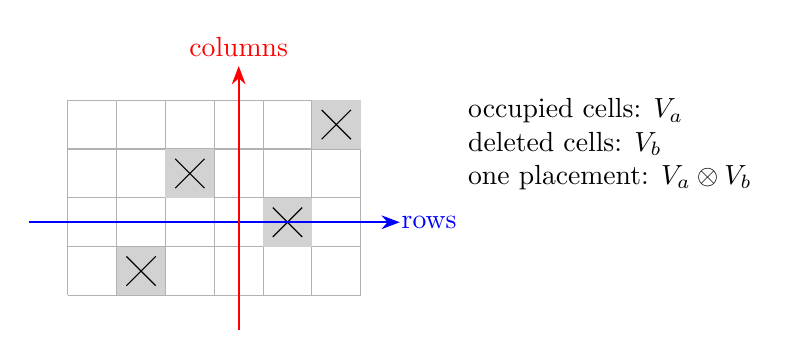
\begin{tikzpicture}[scale=.62]
\foreach \x in {0,...,6} {\draw[gray!60] (\x,0)--(\x,4);}
\foreach \y in {0,...,4} {\draw[gray!60] (0,\y)--(6,\y);}
\foreach \x/\y in {1/0,4/1,2/2,5/3} {\fill[gray!35] (\x,\y) rectangle ++(1,1);\draw (\x+.2,\y+.2)--(\x+.8,\y+.8);\draw (\x+.2,\y+.8)--(\x+.8,\y+.2);}
\draw[-{Stealth},thick,blue] (-.8,1.5)--(6.8,1.5);
\draw[-{Stealth},thick,red] (3.5,-.7)--(3.5,4.7);
\node[blue] at (7.4,1.5) {rows};\node[red] at (3.5,5.1) {columns};
\node[align=left,anchor=west] at (8,3.1) {occupied cells: $V_a$\\deleted cells: $V_b$\\one placement: $V_a\otimes V_b$};
\end{tikzpicture}
\caption{A board with deleted cells, marked by crosses. The occupied-cell estimate applies to every deletion pattern. Restoring the deleted cells assigns the representation $V_a\otimes V_b$ to each placement; the weight comparison pays for summing over placements. The arrows indicate row and column subgroup actions.}
\label{fig:board}
\end{figure}

Weighted Schatten interpolation then transfers the projection bound
to arbitrary matrices in the row and column Fourier blocks. Its
logarithmic error is independent of the Schatten exponent. Applied to
the two families of smaller sweeps, the bound increases the required
exponent by only a factor $1+C/d$. These factors have bounded product
along successive halvings of $d$. A direct forest estimate covers
diagrams whose first row contains almost every box; a strict norm gap
in finitely many small dimensions starts the induction. This proves
Theorem~\ref{thm:weighted} in Section~\ref{sec:completion}.

\subsection{Two further forms of the overlap estimate}
Section~\ref{ten:frames} keeps track of the number of selected directions
inside each row and column carrier, while including every multiplicity
copy. Its Schatten-$8$ bound has a cost controlled by the number of boxes
below the first row. A separate signed-tensor estimate has a cost
controlled by the number of boxes outside a small hook. The two bounds
cover complementary shapes, and a sparse estimate using short time
windows completes another bounded-exponent induction.

Section~\ref{rec:sec-coherent} instead retains the deleted positions as
an ordered list. Summing squared coefficients over the initial,
intermediate, and final hole lists gives the explicit restoration
factor $e^{3l}\binom Nl$, where $l$ is the number of holes. Its
occupied-cell estimate resolves the row and column projections by averaging
over compact-group orbits of highest-weight vectors
\cite[Section~2]{Perelomov1972}. A minimum-norm argument matches their
averaged one-cell densities to a common density before the row--column
comparison. This normalization is related to the highest-weight capacity
framework of \citet[Sections~2 and~4]{FranksWalter2022}; we prove the
required form locally to keep the loss from missing cells explicit. The
overlap proof and moment induction are given here.
The sparse part uses the partial-deck density and lower-diagram bounds
of \citet[Theorem~6.1 and Proposition~6.3]{OpenAI2026Routing}.

The companion \emph{Random-subspace tests and trace smoothing for
coordinate sweeps} \cite{OpenAI2026RandomSubspace} develops related
trace-smoothing estimates. For symmetric-group and tableau conventions we
follow \citet{Sagan2001,Stanley1999}; branching and content spectra are
also developed by \citet{VershikOkounkov2005}. We use ordinary
Schur--Weyl duality in the form of \citet[Theorem~4.57 and
Corollary~4.59]{etingof}.

Section~\ref{sec:conventions} fixes the common representation conventions.
Part~\ref{part:weighted} constructs the weights, proves the occupied-board
and restoration bounds, and completes the first moment proof and the
mixing deduction. Part~\ref{part:frames} develops the selected-rank frame
estimates and their moment induction. Part~\ref{part:coherent} proves
the ordered-hole estimate and closes the coherent-state induction using
the cited partial-deck input.

\section{Representations and subgroup projections}\label{sec:conventions}
Throughout, logs used in estimates are natural logs. We write \(G_L\) for the symmetric group of degree \(L\); spaces can equally well be indexed by sets of size \(L\). Denote the representation belonging to a partition \(\lambda\) by \(V_\lambda\), and its dimension by \(D_\lambda\). We also write \(V_\mu,D_\mu\) for an irreducible of a product group and its dimension. We take the group of degree 0 to be trivial, and allow empty partitions where appropriate. All representations are taken unitary (over \(\mathbb C\)). The trace and Schatten norms on a single matrix space use unnormalized trace unless otherwise indicated. We use \(\|M\|_p=(\operatorname{Tr}|M|^p)^{1/p}\), including operator norm at \(p=\infty\).

We use the following characteristic-zero facts and normalization conventions.
\begin{itemize}
\item We use tableau dimensions, the branching rule, and the hook-length formula for symmetric groups \cite[Theorems~2.6.5, 2.8.3, and~3.10.2]{Sagan2001}. Thus restriction to a symmetric group of smaller degree has shapes given by box deletions. Transposition of a partition corresponds to tensoring with the sign \cite[Theorem~6.7]{James1978}, and induction from two factors of a Young subgroup uses the Littlewood--Richardson coefficients \cite[Theorem~16.4]{James1978}.
\item We will also use ordinary Schur--Weyl duality on a complex tensor power, with the unitary group action on the factors and permutations of slots \cite[Theorem~4.57 and Corollary~4.59]{etingof}. For a local dimension \(h\), the factors in the decomposition for tensor degree \(l\) are the polynomial unitary-group representation with highest weight \(\gamma\) and \(V_\gamma\), for \(\gamma\vdash l\) of length at most \(h\). We use Schur characters in their semistandard-tableau form \cite[Definition~7.10.1]{Stanley1999}. In particular a positive operator acting identically in the slots has, on type \(\gamma\), largest eigenvalue given by the monomial of exponents \(\gamma\) on its eigenvalues sorted in decreasing order. This follows also by column strictness in the tableaux and the presence of the highest weight. The statement for zero eigenvalues can be taken by a limit.
\item Given an irreducible \(\mu\) of a subgroup \(R\) and a matrix \(M\) on \(V_\mu\), we can use a group algebra element of \(R\) with matrix \(M\) there, and zero matrix on its other types, viewed also in any larger group. Its coefficient at \(g\in R\) is
\[
 \frac{D_\mu}{|R|}\operatorname{Tr}\big(M \rho_\mu(g^{-1})\big),
\]
where \(\rho_\mu\) denotes the representation. We refer to the images of this element as matrix actions supported on \(\mu\). For \(M\) the orthogonal projector onto a unit vector \(e\), denote such an image by \(P_{\mu,e}\), specifying or taking as understood the ambient representation. On restriction to \(R\), this is an orthogonal projection using one direction of the carrier and acting identically on the corresponding multiplicity space. A full isotypic projection instead uses \(I_{V_\mu}\). We use the standard orthogonality and Plancherel formulas. In particular the sum of squared absolute values of the above coefficients is \(D_\mu\operatorname{Tr}(M^*M)/|R|\).
\end{itemize}

Write \(K_d(\lambda)\) for the Fourier matrix (expectation of the representing matrix) on \(V_\lambda\), \(\lambda\vdash N\), \(N=2^d\). The length of any partition we need to consider with \(K_d(\lambda)\ne 0\) is at most \(N/2\): one matching of switches already projects to invariants of a Young subgroup with \(N/2\) parts of size 2. The corresponding permutation module only has partitions of length at most \(N/2\) (for example, it occurs in an ordinary slot permutation tensor power with local dimension \(N/2\)).


\part{Weighted contraction}\label{part:weighted}

\section{Dimensions away from a long first row}
\label{ten:weighted:part:53}
Write $k=N-\lambda_1$ for the number of boxes below the first row. The following dimension estimate will be used in all three moment arguments.
\begin{lemma}\label{lem:surviving-dimension}
There is an absolute constant $c>0$ such that, for every $N\ge2$ and every partition $\lambda\vdash N$, $\lambda\ne(N)$, with at most $N/2$ rows,
\[
 \log D_\lambda\ge c(N-\lambda_1).
\]
\end{lemma}
\begin{proof}
First take $N$ sufficiently large. If both the width and the height are less than $N/10$, every hook length is at most $N/5$, and the hook formula gives $\log D_\lambda\ge cN\ge ck$.
Otherwise work in $\lambda$ or its transpose so the first row has size $u\ge N/10$. Let $v=N-u$ be the number of boxes outside that row. In the original orientation $v=k$; in the transposed orientation the height assumption gives $v\ge N/2$. Retain that row and a subdiagram of size $l=\min(v,\lfloor u/2\rfloor)$ below it. In either orientation $l\ge c_1k$ for an absolute $c_1>0$ and large $N$. By branching its dimension is a lower bound for $D_\lambda$. The hook formula bounds this dimension below by
\[
 \binom{u+l}{l}\exp\!\left(-\frac{l}{u-l+1}\right).
\]
Indeed the lower diagram has dimension at least one, its width is at most $l$, and its column heights sum to $l$, so the logarithm of the extra top-row hook factor is at most $l/(u-l+1)$. Since $l\le u/2$, the displayed lower bound has logarithm at least $(\log3-1)l\ge c_2k$. This proves the claim for large $N$. The remaining sizes are finite; decreasing $c$ covers them because the only one-dimensional irreducibles are the trivial and sign representations, both excluded by the hypotheses.
\end{proof}
In particular, for fixed small \(\epsilon>0\), if \(k>N^{1-\epsilon}\) and \(\lambda\) has length at most \(N/2\), then
\begin{equation}
 \log D_\lambda \ \ge\ c_0 N^{1-\epsilon}.                                                  \label{ten:weighted:eq:3}
\end{equation}


\section{Weights from hook trimming}
\label{ten:weighted:part:60}
The weights balance the dimension of a subdiagram against the number of boxes removed. Their parent--child difference will pay for the entropy of restoring deleted cells, while retaining a favorable dimension term. For $L\ge2$, fix
\[
 b_0=\tfrac14,\quad\delta=\tfrac1{16},\quad
 b_1=b_0\delta/4,\quad A=10,\quad
 \eta=b_1/(2A),\quad\epsilon=\eta/8,
\]
and define
\[
 F_L(r)=r\min\{\log(L/r),\eta\log L\}\quad(1\le r\le L),
 \qquad F_L(0)=0.
\]
For a Young diagram $\lambda\vdash L$, a subdiagram $a\subseteq\lambda$ is itself a Young diagram. Put
\begin{equation}\label{ten:weighted:eq:4}
 \begin{split}
 J(\lambda)&=\min_{a\subseteq\lambda}
 \{b_0\log D_a+b_1r\log L-AF_L(r)\},\qquad r=L-|a|,\\
 W_\lambda&=D_\lambda e^{-J(\lambda)}.
 \end{split}
\end{equation}
Empty diagrams have dimension one. For sizes zero and one put $J=0$ and $W=1$. Since $AF_L(r)\le(b_1/2)r\log L$, the expression minimized is nonnegative; taking $a=\lambda$ gives
$0\le J(\lambda)\le\frac14\log D_\lambda$.

On a tuple of partitions for a product of same-size groups, we sum the $J$ values and multiply the $W$ values. We next show that the minimizing subdiagram can be chosen in a hook at a controlled cost.

We will need that at \(L=N\), at additive cost at most \(O(h^2)\) in the minimum of \eqref{ten:weighted:eq:4}, we can take \(a\) in the \(h,h\)-hook, i.e. with no box of indices \(i>h,\ j>h\), for \(h=\lfloor N^\delta\rfloor\) and \(N\) sufficiently large. To show it, take a minimizing partition \(a_1\) and trim off the boxes with both indices \(>h\) leaving \(a\). Write \(x\) for the number trimmed and \(M=|a_1|\), supposing \(x>0\). The hook length formula gives
\begin{equation}
 \log D_{a_1}-\log D_a \ \ge\ x(\log h-C)-C h^2.                                            \label{ten:weighted:eq:5}
\end{equation}
Here the log factorial gain for \(a_1\) is at least \(x(\log M-1)\), and hooks in the trimmed boxes are at most \(2M/h\). Hooks within \(a\) changing length due to horizontal extensions are bounded in their log ratio sum by
\[
 \sum_{i=1}^{p}\sum_{j=1}^{h}\log\left(1+\frac{x_i}{h-j+1+p-i}\right),
\]
where \(p\) is the number of rows of the trimmed portion and \(x_i\) their lengths within that portion, decreasing weakly. If \(p\ge h\), linearize by \(\log(1+v)\le v\), and use that the sum of reciprocals over \(j\) increases with \(i\); its average over \(i\) is at most 2 (bound the double sum of reciprocals by extending to \(p\) columns and summing on diagonals). Thus pairing with decreasing \(x_i\) gives a bound \(2x\). If \(p<h\), the sum of the row contributions is at most
\[
 \sum_{i=1}^p\log\binom{h+x_i}{x_i}
 \le (ph+x)\log2\le(h^2+x)\log2.
\]
The transpose handles vertical extensions. This proves \eqref{ten:weighted:eq:5}. The change upwards in \(b_1 r\log N-A F_N(r)\) from increasing \(r\) by \(x\) is at most \((b_1\log N+A)x\), by the bound \(-1\) on how negative a slope of \(F_N\) can be. Since \(b_1<b_0\delta\), the asserted near-minimum property follows.

For such an \(a\), put \(t=N-|a|\). We will use
\begin{equation}
 b_0\log D_a + b_1 t\log N-A F_N(t)=J(\lambda)+O(h^2),\qquad
 t\log N\le C(\log D_\lambda+h^2),                                                        \label{ten:weighted:eq:6}
\end{equation}
where the second estimate uses the cap in \(F_N\). We allow the empty partition, with dimension 1.

We next prepare an estimate for transverse decompositions of a representation in this hook. This will later be used on a set of cells of a grid excluding \(t\) cells.


\section{Signed representations on occupied cells}
\label{ten:weighted:part:96}
\begin{theorem}[Overlap on an arbitrary occupied board]\label{thm:occupied}
Take a grid with \(m\) rows and \(n\) columns, \(mn=N\), and consider any subset of \(s=N-t\) cells, with the group \(G_s\) on those cells. Let \(a\vdash s\) lie in the \(h,h\)-hook, \(1\le h\le N\). Decompose \(V_a\) under the within-row permutation subgroup of \(G_s\), and also (separately) the within-column subgroup. For types \(\sigma,\theta\) of these two groups, let \(I_{\sigma,u}: V_\sigma\to V_a\), \(I_{\theta,v}: V_\theta\to V_a\) be isometric embeddings giving orthogonal copies and spanning the respective isotypic spaces. Then
\begin{equation}
 \sum_{u,v}\|I_{\sigma,u}^* I_{\theta,v}\|_\infty^2
 \ \le\
 \exp\{C[(m+n+1)h^2\log(N+2)+t]\}\ \min\left\{1,\frac{D_\sigma D_\theta}{D_a}\right\}.       \label{ten:weighted:eq:7}
\end{equation}
Here \(\sigma\) and \(\theta\) can each consist of a tuple of partitions, and the infinity norm is the operator norm. For \(s=0\) the empty representation has dimension one.
\end{theorem}
\begin{proof}
For \(s=0\) the assertion is immediate.

The signed realization uses ordinary Schur--Weyl duality \cite[Theorem~4.57 and Corollary~4.59]{etingof}, sign twist and induction \cite[Theorems~6.7 and~16.4]{James1978}. To prove the estimate we use a slot space
\(\mathcal L=(\mathbb C^h\oplus\mathbb C^h)^{\otimes s}\), calling the two blocks even and odd. Use the signed permutation action: on permuting a tensor of definite parities give the sign of reordering the subsequence of odd slots. This defines a group action (the signs compose), commuting with the global \(U(h)\times U(h)\) action for the two blocks. For clarity, the structure needed here follows from ordinary Schur-Weyl duality. Separate out the slots of even and odd parity. At fixed parity counts \(s_e,s_o\), the action of \(G_s\) moves the allocation of those counts to the slots, and at a fixed allocation the stabilizer action is unsigned permutation on the even slots and sign-twisted permutation on the odd slots. Consequently a \(U(h)\times U(h)\) sector of types \(\gamma,\xi\) (\(|\gamma|=s_e,|\xi|=s_o\), both lengths \(\le h\)) has multiplicity space giving, as a \(G_s\) representation,
\begin{equation}
 \operatorname{Ind}_{G_{s_e}\times G_{s_o}}^{G_s}\big(V_\gamma\otimes V_{\xi^{\rm tr}}\big).   \label{ten:weighted:eq:8}
\end{equation}
Here \(\xi^{\rm tr}\) denotes the transposed partition, and we use ``sector'' with its unitary-group carrier as well as the multiplicity space. There is such a sector containing \(V_a\): take \(\gamma\) from the first \(h\) rows and \(\xi^{\rm tr}\) the remaining rows (a diagram of width at most \(h\)). Indeed \(a/\gamma\) is a straight partition up to shift, so the Littlewood-Richardson coefficient in \eqref{ten:weighted:eq:8} is positive.

Here are size and entropy estimates used with these sectors, applying just as well at any number \(l\le s\) of slots. The dimensions of the unitary-group carriers and the number of sectors are \(\exp(O(h^2\log(N+2)))\), as upper bounds; for dimensions this follows for example by counting the possible counts of each symbol in each row of a semistandard tableau. The multiplicity of any \(\chi\vdash l\) for the signed permutation action on the \(l\) slots is also at most \(\exp(O(h^2\log(N+2)))\). Indeed, for a pair \(\gamma,\xi\) giving a nonzero induction coefficient at \(\chi\), use Littlewood-Richardson fillings of \(\chi/\xi^{\rm tr}\) with content \(\gamma\), and thus entries at most \(h\). Since \(\xi^{\rm tr}\) has width at most \(h\), every skew column beyond column \(h\) is a full column of \(\chi\). Column strictness therefore places these columns within the first \(h\) rows, where the fillings are determined by row counts of symbols. In the first \(h\) columns the skew shape has at most \(h^2\) boxes. These bounds along with \eqref{ten:weighted:eq:8} give the multiplicity estimate.

If \(|\gamma|+|\xi|=l\), write
\[
 H(\gamma,\xi)=\sum_i\gamma_i\log(l/\gamma_i)+\sum_j\xi_j\log(l/\xi_j)
\]
with zero contributions understood at count 0. For the same occurrence of \(\chi\), we have
\begin{equation}
 D_\chi\ \le\ \exp(H(\gamma,\xi))\ \le\ D_\chi\exp(C h^2\log(N+2)).                         \label{ten:weighted:eq:9}
\end{equation}
For the first bound use \(D_\chi\le\binom{l}{|\gamma|}D_\gamma D_\xi\), by \eqref{ten:weighted:eq:8} and invariance of dimension under transposition, and bound each factor by the multinomial of its row lengths. For the second bound, \(\chi\) is in the \(h,h\)-hook and contains both \(\gamma\) and \(\xi^{\rm tr}\). Since \(|\gamma|+|\xi^{\rm tr}|=|\chi|\), the number of boxes of \(\chi\) outside their union equals \(|\gamma\cap\xi^{\rm tr}|\), which is at most \(h^2\). In particular the total excess of its first \(h\) row lengths over the corresponding \(\gamma_i\) is \(O(h^2)\), and similarly for the first \(h\) column lengths and \(\xi_j\). In bounding its product of hooks, the part in its first \(h\) rows beyond column \(h\) has leg lengths bounded by \(h\), and the analogous statement for arms applies below its first \(h\) rows. This gives an upper bound on the hook product of
\[
 (N+2)^{C h^2}\prod_i\gamma_i!\prod_j\xi_j!
\]
(for example, for the horizontal part use the top row factorials, increasing their arguments by at most \(h\) in each row, and likewise for columns in the vertical part). Stirling's bound, or the elementary multinomial entropy bounds, now gives \eqref{ten:weighted:eq:9}.


\subsection{Two bounds for transverse overlap}
\label{ten:weighted:part:127}
We now prove the two bounds whose minimum occurs in Theorem~\ref{thm:occupied}. Counting copies gives the first; positive states and two-sided normalization give the dimension ratio.

We already get a bound \(\exp(O((m+n)h^2\log(N+2)))\) on the number of matrices \(I_{\sigma,u}^*I_{\theta,v}\), hence also on the sum in \eqref{ten:weighted:eq:7}, by using the multiplicity estimate row by row and column by column in \(\mathcal L\). When grouping slots for a subgroup, we can rearrange them with the signed reordering, after which contiguous block permutations give the tensor product actions. It remains to get the other bound in \eqref{ten:weighted:eq:7}. Let $P_\sigma,P_\theta$ be the isotypic projections on $V_a$. The all-copy identity
\[
 \sum_{u,v}\|I_{\sigma,u}^*I_{\theta,v}\|_2^2
 =\operatorname{Tr}_{V_a}(P_\sigma P_\theta)
\]
follows by expanding each projection as the sum over its orthogonal embeddings. We bound this sum of squared Hilbert--Schmidt norms, which also bounds the required sum of squared operator norms. Use a global unitary-group sector containing \(V_a\) as above, with projector \(P\) in \(\mathcal L\), and types denoted by \(\gamma,\xi\). If \(Q_\sigma,Q_\theta\) denote the subgroup isotypic projections on \(\mathcal L\), the trace we need to estimate is bounded by
\[
 \operatorname{Tr}_{\mathcal L}(Q_\sigma P Q_\theta P).
\]
Indeed \(P\) commutes with the permutations and each \(G_s\)-irreducible contribution to the trace on that sector is nonnegative.

We can majorize \(Q_\sigma\) in positive semidefinite order by a mixture of products \(S\) of states on individual slots, using the same state \(S_i\) in every slot of row \(i\), each state even (block diagonal). Here and below a state is positive semidefinite with trace 1. The scalar prefactor for this majorization can be taken to be \(D_\sigma\exp(Cm h^2\log(N+2))\), with the mixture a probability mixture. To see this on one row of size \(l>0\), bound the projection for its partition \(\chi\) by the sum of sector projections for compatible \((\gamma_0,\xi_0)\) at \(l\) slots. In each case twirl, by the unitary group \(U(h)\times U(h)\), the identical-slot product of a block diagonal state with diagonal entries \((\gamma_{0,i}/l,\xi_{0,j}/l)\). It acts after twirling as a scalar on this sector, at least \(\exp(-H(\gamma_0,\xi_0))\) divided by the dimension of the unitary-group carrier. Indeed before twirling it has the eigenvalue given by the highest weight and acts as identity on multiplicities in the sense of a matrix action on the carrier tensored with identity. This latter action of an identical even positive matrix in tensor power follows directly from ordinary Schur-Weyl on the two parities (and by limits for singular matrices). The twirl is positive on the other sectors. Now the bound on the prefactor follows from \eqref{ten:weighted:eq:9} and the counting and dimension bounds. A size-zero row requires nothing and can use any even state for its specification. The same majorization applies to \(Q_\theta\), with products \(T\) using \(T_j\) in column \(j\), and prefactor \(D_\theta\exp(C n h^2\log(N+2))\). Even when undoing a signed reordering of slots, such products are ordinary products since their factors preserve the local parity. Thus by two positive semidefinite majorizations (tracing with the other positive matrix conjugated by \(P\)), we can use bounds on
\(\operatorname{Tr}_{\mathcal L}(S P T P)\).

The normalization has two purposes: the global sector operator must contribute $\exp(-H(\gamma,\xi))$ to the squared norm, and the local overlaps must have mean at most one under the independent row and column marginals. Quarter-root filters meet both requirements. For fixed \(S,T\) so specified, let \(\bar S,\bar T\) be the average one-slot states over the \(s\) cells in consideration, and put \(X=\bar S^{1/2}\), \(Y=\bar T^{1/2}\). Write
\[
 S_i'=X^{-1/2} S_i X^{-1/2},\qquad T_j'=Y^{-1/2}T_jY^{-1/2}
\]
with inverses on supports. Let \(S',T'\) be the corresponding products, so the filtering can be undone using \(X^{1/2},Y^{1/2}\) on occupied slots. With
\[
 L=(X^{1/2})^{\otimes s} P (Y^{1/2})^{\otimes s}
\]
we have
\[
 \operatorname{Tr}_{\mathcal L}(S P T P)=\|(S')^{1/2} L (T')^{1/2}\|_2^2 .
\]
The matrix action \(L\) is supported on the \((\gamma,\xi)\) unitary-group sector with operator norm at most \(\exp(-H(\gamma,\xi)/2)\). Indeed \((X^{1/2})^{\otimes s}=(\bar S^{1/4})^{\otimes s}\) acts on this sector with norm at most \(\exp(-H(\gamma,\xi)/4)\), by taking largest weight monomials on the eigenvalues and using that the eigenvalues of \(\bar S\) sum to 1. The same argument applies with \(\bar T\). These matrix actions are identical on equivalent copies for the block unitary group. By matrix coefficient orthogonality for that compact group, \(L\) can therefore be represented by an integral of the global \(U^{\otimes s}\) for block unitaries \(U\), with coefficient function bounded by \(\|L\|_\infty\) times the squared carrier dimension. (This is the matrix Fourier formula for an action supported on one type.)

For each block unitary define \(z_{ij}=\operatorname{Tr}(S_i' U T_j' U^*)\). The squared Hilbert-Schmidt norm weighted by \(S',T'\), as above but for \(U^{\otimes s}\), is the product of \(z_{ij}\) over the cells under consideration. If \(p_i,q_j\) are the marginals of a uniformly chosen cell among these \(s\), the mean of \(z_{ij}\) under \(p_i q_j\) is at most 1. In fact it is \(\operatorname{Tr}(\bar S^{1/2} U\bar T^{1/2}U^*)\), at most 1 by Cauchy-Schwarz. Under the actual uniform law on the cells the mean of \(\log z_{ij}\) is thus bounded above by the relative entropy of that law with respect to \(p_i q_j\), by the elementary entropy variational inequality (the entropy/product duality is discussed in \cite[Theorem~2.1 and (2.4)]{CarlenCorderoErausquin2009}). Explicitly, if $\omega$ is the occupied-cell law and $r_{ij}=p_iq_j$, Jensen applied to $\sum\omega_{ij}\log(z_{ij}r_{ij}/\omega_{ij})$ gives at most $\log\sum r_{ij}z_{ij}\le0$. Zero values in the product need no bound. The relative entropy is at most \(\log(mn/s)\), by bounding the two marginal entropies by \(\log m,\log n\), so the product is at most \(\exp(s\log(N/s))\le\exp(t)\). Using the integral for \(L\) and the triangle inequality, we obtain
\[
 \operatorname{Tr}_{\mathcal L}(S P T P)
 \ \le\ \exp\{C h^2\log(N+2)+t\}\exp(-H(\gamma,\xi)).
\]
Since \(D_a\le\exp(H(\gamma,\xi))\), the mixture prefactors give the required bound with \(D_\sigma D_\theta/D_a\) in \eqref{ten:weighted:eq:7}, completing the proof.
\end{proof}


\section{The row-column Fourier estimate}
\label{ten:weighted:part:157}
Split a sweep of dimension \(d\) into two parts, each scanning consecutive coordinates, with block sizes \(d_1=\lfloor d/2\rfloor\) and \(d_2=d-d_1\). Index positions as a grid, so these parts use the within-row and the within-column subgroups, denoted \(R,C_{\rm col}\). Write \(n\) for the size of a row and \(m\) for that of a column, so \(mn=N\), \(m,n\) both within a constant factor of \(\sqrt N\). We take \(d\) large. Suppose henceforth in the estimate that
\begin{equation}
 k=N-\lambda_1>N^{1-\epsilon},\qquad \lambda^{\rm tr}_1\le N/2.                            \label{ten:weighted:eq:10}
\end{equation}

For irreducibles \(\mu,\nu\) of \(R,C_{\rm col}\), each a tuple, and unit carrier vectors \(e,f\), we claim the following bound on projections in \(V_\lambda\):
\begin{equation}
 W_\lambda\operatorname{Tr}_{V_\lambda}(P_{\mu,e}P_{\nu,f})
 \ \le\ W_\mu W_\nu\exp\{O((\log D_\lambda)/d)\}.                                          \label{ten:weighted:eq:11}
\end{equation}
All constants are independent of the types and of \(d\).

Use the hook \(a\) from \eqref{ten:weighted:eq:6} and choose a partition \(b\vdash t\) such that
\[
 \mathcal I=\operatorname{Ind}_{G_{N-t}\times G_t}^{G_N}(V_a\otimes V_b)
\]
contains \(V_\lambda\), possible by branching and decomposing the restriction. We bound the trace of \(X Y\) on \(\mathcal I\), for \(X=P_{\mu,e}\), \(Y=P_{\nu,f}\) acting here; this bounds the desired trace before multiplying by \(W_\lambda\), as the trace on each contributing \(G_N\)-type is nonnegative. Use the direct sum structure of \(\mathcal I\) with a fiber at each \(t\)-set \(Z\) of the grid. Its stabilizer acts on this fiber by \(V_a\) on the complement and \(V_b\) on \(Z\).

Let \(v_i\) be the counts of \(Z\) in rows and \(u_j\) in columns. The full row and column orbit sizes and overall size we denote by
\[
 L_R=\prod_i\binom n{v_i},\qquad L_C=\prod_j\binom m{u_j},\qquad L_0=\binom Nt.
\]
Let \(L_{RC}\) be the number of sets with the indicated two profiles. Use untruncated quantities
\[
 H_R=\sum_i v_i\log(n/v_i),\quad H_C=\sum_j u_j\log(m/u_j),\quad H_0=t\log(N/t),
 \quad E_0=H_R+H_C-H_0.
\]
Here again terms at zero count are zero. For nonempty layout classes \(E_0\ge 0\); for \(t>0\) it is \(t\) times the relative entropy of the uniform distribution on \(Z\) with respect to the product of its marginals. We have
\begin{equation}
 \log \frac{L_{RC}^2 L_0}{L_R L_C}\le E_0+O(t).                                            \label{ten:weighted:eq:12}
\end{equation}
Indeed \(\log L_R\ge H_R,\log L_C\ge H_C,\log L_0\le H_0+t\) by binomial bounds. For a uniform random set with the two profiles, subadditivity bounds \(\log L_{RC}\) by the sum of marginal indicator entropies. To bound that sum, choose a cell uniformly and call its indices \(I,J\) and its random indicator \(V\). As \(I,J\) are independent,
\[
 H(V\mid I,J)\le H(V\mid I)+H(V\mid J)-H(V)
\]
in ordinary entropy notation (by nonnegativity of conditional mutual information). Multiplying by \(N\), the terms on the right give an upper bound at most \((H_R+t)+(H_C+t)-H_0\), since the complementary term to \(v_i\log(n/v_i)\) in row binary entropy times row size is at most \(v_i\), and similarly for columns. Thus $\log L_{RC}\le E_0+2t$. Combining this with the three binomial bounds gives
\[
 2\log L_{RC}+\log L_0-\log L_R-\log L_C\le E_0+5t,
\]
which proves \eqref{ten:weighted:eq:12}.


\subsection{Positive blocks and stabilizer coefficients}
\label{ten:weighted:part:194}
The block trace for \(X Y\) only uses pairs \(Z,Z'\) with both profiles the same between them. In bounding the absolute sum of block contributions for one layout class, we can use \(L_{RC}^2\) times the maximum diagonal-block overlap \(\operatorname{Tr}(X_{ZZ}Y_{ZZ})\) in that class. In fact an off-diagonal block of a positive matrix has the form \(X_{ZZ}^{1/2} U X_{Z'Z'}^{1/2}\) for a contraction \(U\), and likewise for \(Y\); thus \(|\operatorname{Tr}(X_{ZZ'}Y_{Z'Z})|\) is bounded using Hilbert-Schmidt by the geometric mean of the corresponding diagonal-block overlap traces.

For fixed \(Z\), the row stabilizer \(R_Z\) in \(R\) acts separately on its sites outside and inside \(Z\). Write its types as \(\alpha=(\sigma,\tau)\) for the two parts respectively. The diagonal block \(X_{ZZ}\) has the following formula: on the fiber it is
\begin{equation}
 \frac{D_\mu}{L_R}\sum_{\alpha}\frac{1}{D_\alpha}\, \mathcal P_{\alpha,M_\alpha}.             \label{ten:weighted:eq:13}
\end{equation}
Here \(\mathcal P_{\alpha,M_\alpha}\) denotes a matrix action supported on \(\alpha\) for \(R_Z\), where the \(M_\alpha\) are positive matrices of total trace 1. More explicitly, write
\[
 V_\mu\!\downarrow_{R_Z}=\bigoplus_\alpha V_\alpha\otimes\mathcal M_{\mu,\alpha},\qquad
 e=\bigoplus_\alpha e_\alpha,\qquad
 M_\alpha=\operatorname{Tr}_{\mathcal M_{\mu,\alpha}}|e_\alpha\rangle\langle e_\alpha|.
\]
Then $M_\alpha\succeq0$ and $\sum_\alpha\operatorname{Tr}M_\alpha=\sum_\alpha\|e_\alpha\|^2=1$. Keeping just permutations in $R_Z$ in the matrix coefficient formula for $P_{\mu,e}$, and using $|R|=L_R|R_Z|$, gives \eqref{ten:weighted:eq:13} by orthogonality. The multiplicity spaces have been traced out, not counted. Similarly for \(Y_{ZZ}\) we use column stabilizer types \(\zeta=(\theta,\pi)\) with factor \(D_\nu/L_C\). Only types occurring in the corresponding restrictions and the fiber need be considered.

The positive states in \eqref{ten:weighted:eq:13} need not be product states on the surviving and deleted carriers. The following elementary estimate is the reason this causes no extra dimension factor.
\begin{lemma}[Arbitrary carrier vectors]\label{lem:entangled}
Let \(A_i:E^\prime\to E\) and \(B_j:F^\prime\to F\) be finite families of operators between finite-dimensional Hilbert spaces. Suppose
\[\sum_j|\langle x,B_jy\rangle|^2\le C\|x\|^2\|y\|^2.\]
Then for unit \(w\in E\otimes F\), \(w^\prime\in E^\prime\otimes F^\prime\),
\[\sum_{i,j}|\langle w,(A_i\otimes B_j)w^\prime\rangle|^2\le C\sum_i\|A_i\|_\infty^2.\]
\end{lemma}
\begin{proof}
For fixed \(i\), the functional \(B\mapsto\langle w,(A_i\otimes B)w^\prime\rangle\) has norm at most \(\|A_i\|_\infty\) on the operator-norm space. By trace-norm duality and singular-value decomposition it is a sum \(\sum_s c_s\langle x_s,By_s\rangle\), where \(x_s,y_s\) are unit vectors, \(c_s\ge0\), and \(\sum_s c_s\le\|A_i\|_\infty\). The triangle inequality in \(\ell^2(j)\) bounds the corresponding square root by \(\sqrt C\sum_s c_s\). Square and sum over \(i\).\end{proof}

For these fiber actions, take any pure unit states on the carriers \(V_\sigma\otimes V_\tau\) and \(V_\theta\otimes V_\pi\), denoted by \(w,w'\) as vectors. The corresponding overlap trace on the fiber is of the form
\begin{equation}
 \sum_{l,r} |\langle w,(A_l\otimes B_r) w'\rangle|^2.                                      \label{ten:weighted:eq:14}
\end{equation}
Here \(A_l\) range over the products \(I_{\sigma,u}^* I_{\theta,v}\) for the two decompositions of \(V_a\) as in \eqref{ten:weighted:eq:7}, and \(B_r\) analogously use \(V_b\), for types \(\tau,\pi\). This follows by writing the projection directions in every pair of copies in the restricted representations.

On \(Z\) itself, the within-row and within-column groups have trivial intersection. For unit vectors \(x,y\) of the two relevant carriers there, Plancherel gives
\begin{equation}
 \sum_r |\langle x,B_r y\rangle|^2
 \ \le\ \frac{D_\tau D_\pi}{D_b}\frac{t!}{\prod_i v_i!\prod_j u_j!}
 \ \le\ \frac{D_\tau D_\pi}{D_b}\exp(E_0+O(t)).                                             \label{ten:weighted:eq:15}
\end{equation}
Indeed the sum is a trace of a product of projections on \(V_b\), hence also the squared Hilbert-Schmidt norm of the product. The squared group-coefficient sum for the product of the two subgroup matrix elements used to give the projections (as group algebra elements) is the product of their squared coefficient sums, since the pairwise products of group elements use unique factorizations from those two subgroups. This gives the first bound using Plancherel in \(G_t\). The log factorial ratio is bounded as stated using \(E_0=t\log t-\sum_i v_i\log v_i-\sum_j u_j\log u_j\) and elementary factorial bounds.

Lemma~\ref{lem:entangled} bounds \eqref{ten:weighted:eq:14} by the right side of \eqref{ten:weighted:eq:15} times \(\sum_l\|A_l\|_\infty^2\), for arbitrary, possibly entangled, carrier vectors. We next keep the gain from the minimum in Theorem~\ref{thm:occupied}; it is needed when the placement entropy is paid.

Denote
\[
 S=\max\{0,\log(D_\sigma D_\theta/D_a)\}.
\]
Using \eqref{ten:weighted:eq:7}, \eqref{ten:weighted:eq:14}, and \eqref{ten:weighted:eq:15}, after dividing by \(D_\alpha D_\zeta\) from the diagonal-block formulas, the pure-state bound becomes
\begin{equation}
 \frac{1}{D_aD_b}
 \exp\{E_0-S+O(t+(m+n+1)h^2\log(N+2))\}.                                                  \label{ten:weighted:eq:16}
\end{equation}
The matrices within \eqref{ten:weighted:eq:13} and the column counterpart are handled by positive combinations of the pure states with total weights 1. Thus we can take upper bounds for the possible stabilizer types without a count-factor here. Multiplying by \(D_\mu D_\nu L_{RC}^2/(L_R L_C)\), and using \(D_\lambda\le L_0 D_a D_b\) and \eqref{ten:weighted:eq:12}, bounds the overlap for each layout class using \eqref{ten:weighted:eq:16}, by a bound of the form
\begin{equation}
 \frac{D_\mu D_\nu}{D_\lambda}
 \exp\{2E_0-S+O(t+(m+n+1)h^2\log(N+2))\},                                                 \label{ten:weighted:eq:17}
\end{equation}
taking the largest needed over contributing types.


\subsection{The budget pays for layout entropy}
\label{ten:weighted:part:234}
The restored-cell estimate still contains the cost \(2E_0-S\). We now compare it with the difference between the parent and child diagram weights.

To apply \eqref{ten:weighted:eq:4}, each \(\sigma_i\) for a complement row of size \(n-v_i\) is a subpartition of \(\mu_i\), due to restriction, and likewise \(\theta_j\subseteq\nu_j\) has size \(m-u_j\). Hence, denoting the sums of \(J\)'s by \(J(\mu),J(\nu)\), we have
\[
 J(\mu)+J(\nu)\ \le\
 b_0\log(D_\sigma D_\theta)+b_1 t\log N
 -A\left(\sum_i F_n(v_i)+\sum_j F_m(u_j)\right).
\]
Together with \eqref{ten:weighted:eq:6} this gives
\begin{equation}
 J(\lambda)-J(\mu)-J(\nu)
 \ \ge\ -b_0 S + A E_0 -O\big(h^2+(m n^{1-\eta}+n m^{1-\eta})\log(N+2)\big).               \label{ten:weighted:eq:18}
\end{equation}
Indeed the cap in the parent \(F_N\) term does not hurt this lower bound, and the amounts dropped from the row contributions to \(H_R\) come only from positive \(v_i\) less than \(n^{1-\eta}\), with a similar bound for \(H_C\).

Indeed, if $\mathcal E$ denotes the error on the right of \eqref{ten:weighted:eq:18}, then
\[
 2E_0-S-[J(\lambda)-J(\mu)-J(\nu)]
 \le (2-A)E_0-(1-b_0)S+\mathcal E\le\mathcal E.
\]
Here $A\ge2$, $b_0\le1$, and $E_0,S\ge0$. Thus the negative dimension term survives the off-diagonal count and is exactly strong enough when the ratio $D_\mu D_\nu/D_\lambda$ is replaced by $W_\mu W_\nu/W_\lambda$. All the log errors so far and the log count of possible profile choices, the latter \(O((m+n)\log(N+2))\), are bounded by \(O((\log D_\lambda)/d)\). Indeed \(t\) satisfies \eqref{ten:weighted:eq:6}, \(h\le N^{1/16}\), \(m,n\) are of order \(\sqrt N\), and we have \eqref{ten:weighted:eq:3} with \(\epsilon<\eta/2\). These estimates are for all sufficiently large \(d\) under \eqref{ten:weighted:eq:10}. This proves \eqref{ten:weighted:eq:11}.


\section{Weighted Schatten interpolation}
\label{ten:weighted:part:249}
The row part and the column part of the sweep, as group algebra elements, multiply to give \(K_d\) in the order specified by the scan (either product order will be fine for estimates). Within each row, the row part is an independent sweep in its smaller number of bits, and analogously for the columns. This holds because a group of consecutive bit updates in this sweep uses matchings confined to the indicated sets of positions, independently across the sets.

Still under \eqref{ten:weighted:eq:10}, let \(\mathcal B(M,M')\) on \(V_\lambda\) be the product of matrix actions, one for each subgroup, using arbitrary matrices \(M_\mu\) and \(M'_\nu\) on their respective irreducibles. Each subgroup action here is the sum over its irreducibles. By \eqref{ten:weighted:eq:11} we have
\begin{equation}
 W_\lambda \|\mathcal B(M,M')\|_2^2
 \ \le\ \exp\{O((\log D_\lambda)/d)\}
 \left(\sum_\mu W_\mu\|M_\mu\|_2^2\right)\left(\sum_\nu W_\nu\|M'_\nu\|_2^2\right).          \label{ten:weighted:eq:19}
\end{equation}
For a single pair of types this follows by writing the squared norm as a trace of a product of positive matrix actions (using the matrices times their adjoints or the reverse, as appropriate), then diagonalizing and using \eqref{ten:weighted:eq:11}. To sum in \eqref{ten:weighted:eq:19} use the triangle and Cauchy-Schwarz inequalities, absorbing log count factors into the given error. The log counts of the tuples of partitions for the two groups are \(O(N^{3/4}\log(N+2))\), using e.g. the partition count bound \(\exp(O(\sqrt n\log(n+2)))\) (split a partition according to parts of size greater than \(\sqrt n\) and the rest). So \eqref{ten:weighted:eq:3} suffices. Also
\[
 \|\mathcal B(M,M')\|_\infty\le \max_\mu\|M_\mu\|_\infty\ \max_\nu\|M'_\nu\|_\infty
\]
by unitary restriction. For \(2\le p<\infty\), interpolation therefore gives
\begin{equation}
 W_\lambda \|\mathcal B(M,M')\|_p^p
 \ \le\ \exp\{O((\log D_\lambda)/d)\}
 \left(\sum_\mu W_\mu\|M_\mu\|_p^p\right)\left(\sum_\nu W_\nu\|M'_\nu\|_p^p\right),          \label{ten:weighted:eq:20}
\end{equation}
with the coefficient in the log error bounded independently of \(p\).

For details, let $E=C(\log D_\lambda)/d$ be a common logarithmic error bound in \eqref{ten:weighted:eq:19}. The direct-sum Schatten norms use traces weighted blockwise by the given positive numbers and the output norm similarly. The bilinear map has norm at most $e^{E/2}$ at the $2$ endpoint and at most one at the $\infty$ endpoint. Normalize both inputs to norm 1 at \(p\), and test the output using the output weighted trace with a dual-norm-one matrix at \(p'=p/(p-1)\). In the strip with value taken at \(z=2/p\), extend the inputs analytically blockwise using their polar factors and exponent \(p z/2\) on their absolute values (zero singular directions may be kept zero). Their norms on the two boundaries, at \(\infty\) and 2 respectively, are then bounded by 1. Extend the matrix used in the trace test similarly (analytic for the matrix appearing in the trace), with exponent \(p'(1-z/2)\) for boundary norms at 1 and 2. At $\theta=2/p$, the three-lines inequality applied to the weighted trace with the bilinear product gives the factor $e^{(E/2)\theta}=e^{E/p}$. Taking the $p$-th power gives $e^E$ in \eqref{ten:weighted:eq:20}, with no growth of the logarithmic error coefficient in $p$.


\section{Sparse representations and completion}\label{sec:completion}
We have established the matrix inequality needed for the recursive range. A direct estimate handles representations whose first row contains almost all boxes. We prove that estimate here, then close the induction.
\subsection{A sparse forest estimate}
\label{ten:weighted:part:21}
Write \(k=N-\lambda_1\). For \(k\ge 1\) we have the bound
\begin{equation}
 \|K_d(\lambda)\|_\infty \ \le\ (C d)^k (k/N)^{k/8}                                                   \label{ten:weighted:eq:1}
\end{equation}
for an absolute \(C\). We prove it using the sweep kernel \(K\) on ordered injective \(k\)-tuples. Consider the subspace of functions \(f\) of the tuples with sum zero over any one component when all the others are fixed. This space is invariant for the position-permutation action. The module on the tuples contains \(V_\lambda\) by branching (invariants upon restriction to \(G_{N-k}\)). Since \(V_\lambda\) does not occur on \((k-1)\)-tuples, the isotypic space for \(\lambda\) on \(k\)-tuples belongs to the indicated zero-sum subspace. The kernel acts using the sweep in this representation or its adjoint convention.

In a transition \(x\mapsto y\) of tuples, a path for each component is specified just by its start and end: the successive coordinates at the end replace those of the start. For two components, let \(l\) be the last differing bit at the start, and \(r\) the first differing bit at the end. Give this pair weight \(w=0\) if \(r>l\), weight 2 if \(r=l\), and weight 1 otherwise. Then
\[
 K(x,y)=N^{-k}\prod_{\text{pairs}}w.
\]
Indeed, the paths have no conflict (two at the same position at the same stage boundary) exactly when \(r\le l\) for all pairs. When there is no conflict, a switch used by two paths instead of one is used by a pair with \(r=l\), at that bit, giving the factor 2. The same formula works for any subset of components.

Acting on the specified functions \(f\), we can replace the kernel by
\[
 D(x,y)=N^{-k}\sum_{B\subseteq [k]}(-1)^{k-|B|}\prod_{\text{pairs in }B}w,
\]
because all terms for proper subsets use zero marginal sums. This expression vanishes unless the graph of pairs with \(w\ne 1\) has no isolated vertex. Also, its absolute column sums are at most \(2^k\), since each subset term in absolute value uses the nonnegative sweep kernel on that subset (doubly stochastic), with the other start components summed subject to injectivity.

Use this replacement in \(K^* K\), using row \(z\) of \(K^*\) to sample \(x\). For the set \(S\) of positions occupied in \(x\), we have for every fixed set \(F\)
\begin{equation}
 \Pr(S\supset F)\le (k/N)^{|F|}.                                                            \label{ten:weighted:eq:2}
\end{equation}
In fact the upper product-of-marginals bounds for inclusions hold at the start of \(K^*\), which uses a reverse scan, from a fixed tuple \(z\). Such bounds are preserved by a random switch: for an inclusion testing just one of the switched sites, average the two bounds, and for one testing both, their product of marginals at these sites can only increase under averaging. At the end, the marginals are \(k/N\), since a single position is exactly uniform after all bit updates. This is the particular negative-dependence property needed here; stronger preservation results for partial symmetrizations are proved in \cite[Theorems~4.9 and~4.20]{BorceaBrandenLiggett2009}.

For a given \(B\), to bound the row sum using the term with weight product on \(B\) and the no-isolated-vertex condition, use true sweep paths for \(B\) and independent paths with uniform ends for the other components (we can disregard the final injectivity restriction for upper bounding the probability). If \(w\ne 1\), the two specified paths go through the same switch at a stage. We may pre-sample, independently of \(S\), two options at every starting position: a path using a common sweep permutation with its specified routing, and a path from independent uniform bits (independent paths for this option at different positions). Thus we only need upper bound the probability of a no-isolated-vertex interaction graph on \(S\) using some assignment of these types.

Such a graph contains a spanning forest with \(c\le k/2\) rooted trees of size at least 2, which we may take as ordered trees arranged in order of their root positions. The number of forest shapes needed for each \(c\) is at most \(C_0^k\), for an absolute \(C_0\) (e.g. by the traversal encoding of plane forests). Choose distinct roots in at most \(\binom Nc\) ways and path types in at most \(2^k\) ways. For these choices the expected number of embeddings with distinct positions and meetings along the tree edges is at most \((2d)^{k-c}\). To see this, condition on the full common routing and enumerate children after their parents, exposing independent paths as needed. For a child of common routing type, at each possible meeting stage there are at most two starting positions since the full routing sends exactly two paths through the switch. For a child of independent type, summed over fresh positions the expected number meeting a given parent at stage \(i\) is at most \(2^i 2^{-(i-1)}\): the suffix after \(i\) at the start must agree with the parent path there, and the new prefix of length \(i-1\) must agree. These estimates apply to the sums of extension probabilities conditional on the paths for a partial embedding, by independence for unused positions of the independent type. Each embedding uses \(k\) sites, so we may multiply the expected counts by \((k/N)^k\) by \eqref{ten:weighted:eq:2}. Summing over \(B\), shapes and embeddings gives, for the signed kernel \(K^*D\), an absolute row sum bounded by
\[
 (C_1 d)^k (k/N)^{k/2},
\]
using \(\binom Nc\le (C_2 N/k)^{k/2}\) for \(c\le k/2\). An empty set of such forests gives zero probability. The column sum bound for \(D\) still works for \(K^*D\). The row-column sum bound on the \(\ell^2\) operator norm now bounds \(K^*K\) on the specified subspace, proving \eqref{ten:weighted:eq:1}.


\subsection{The bounded-exponent induction}
\label{ten:weighted:part:271}
\begin{proof}[Proof of Theorem~\ref{thm:weighted}]
All sweep matrices are contractions. Partitions of length greater than \(N/2\) need no estimate due to the matching projection, and the trivial one satisfies \eqref{eq:weighted-main} at any exponent. For \(1\le k=N-\lambda_1\le N^{1-\epsilon}\), \eqref{ten:weighted:eq:1} and \(W_\lambda\le D_\lambda\le N^k\) suffice at any exponent at least an absolute sufficiently large constant, for sufficiently large \(d\). Indeed the norm bound \eqref{ten:weighted:eq:1} in this range is at most \(N^{-\epsilon k/16}\) for large \(d\).

For the remaining partitions, suppose \eqref{eq:weighted-main} holds at the two smaller bit sizes in the split. Use \eqref{ten:weighted:eq:20} at \(p=\max(p_{d_1},p_{d_2})\), with the subgroup inputs given by the two subgroup sweep parts. Each input on a tuple of partitions is a tensor product of smaller sweep matrices. Hence each weighted \(p\)-th power term of the inputs is at most 1, and the sums again use only the tuple count bounds. We get
\[
 W_\lambda \|K_d(\lambda)\|_p^p \le \exp(C (\log D_\lambda)/d)
\]
with \(C\) absolute, for all sufficiently large \(d\). In particular \(\|K_d(\lambda)\|_\infty^p\le D_\lambda^{-1/2}\) for these \(d\), by the lower bound on \(W_\lambda\). Increasing \(p\) to \(p(1+C'/d)\) for a large enough absolute \(C'\) gives \eqref{eq:weighted-main}, by using this operator norm on the additional powers.

To implement the induction, take an absolute base threshold on \(d\) sufficiently high for all these estimates. For each of the finitely many base dimensions a nontrivial sweep matrix has operator norm strictly less than 1: it is a product of orthogonal projections from the matchings, and equality of norms on a unit vector would require a common invariant vector for the matching switch subgroups. These generate the symmetric group since all individual edge transpositions of a connected cube are included. Thus a common sufficiently large base exponent can be used for \eqref{eq:weighted-main}, taken large enough for the sparse range as well. Thereafter use the recurrence just given with factor \(1+C'/d\) and the maximum of the two exponents for the split. These exponents are bounded above by an absolute constant since the dimensions in bits along a descent are successively halved up to rounding, so the products of the increment factors stay bounded. This proves the theorem.\end{proof}


\subsection{Full-deck mixing}
\label{ten:weighted:part:285}
In particular for nontrivial \(\lambda\) with length at most \(N/2\) we have
\[
 \|K_d(\lambda)\|_\infty\le D_\lambda^{-(1-b_0)/p_*}.
\]
For an absolute sufficiently large number \(j\) of sweeps, by Plancherel and Cauchy--Schwarz \cite[Sections~2 and~3]{DiaconisShahshahani1981}, the squared total variation distance to uniform of their product law is at most
\[
 \frac14\sum_{\lambda\ne(N)} D_\lambda \|K_d(\lambda)^j\|_2^2
 \ \le\ \frac14\sum_{\substack{\lambda\ne(N)\\ \lambda^{\rm tr}_1\le N/2}} D_\lambda^{-2},
\]
where we took \(j\) large enough for the last exponent, using the operator norm to bound the Hilbert-Schmidt norm. The sum bound tends to zero. Indeed for \(k>N^{1-\epsilon}\) this follows from \eqref{ten:weighted:eq:3} and the partition count, and for \(1\le k\le N^{1-\epsilon}\), \(D_\lambda\ge e^{-1}(N/k)^k\) for large \(N\). The latter follows by the top-row hook estimate in the proof of Lemma~\ref{lem:surviving-dimension}, now with \(k\) boxes outside the row. There are at most \(2^k\) partitions of the tail of size \(k\). Since the permutation product law determines the deck from any fixed starting deck, the bound is a worst-case bound. Thus a fixed number $j$ of sweeps gives total variation distance at most $1/4$ for all sufficiently large $d$. For each of the finitely many remaining $d$, the strict nontrivial Fourier norm gap established above gives convergence under repeated forward sweeps. Increasing $j$ to cover these sizes yields one absolute sweep count for every $d\ge1$; further convolution cannot increase total variation distance. As a sweep consists of $d$ physical shuffles, this proves the upper bound in Corollary~\ref{cor:optimal-mixing}.

\begin{proposition}[Support obstruction]\label{ten:support}
Let $q_d$ be the law of one physical Thorp shuffle. For every integer $t\ge0$, its $t$-fold convolution satisfies
\[
 \|q_d^{*t}-U_{S_N}\|_{\rm TV}\ge1-\frac{2^{tN/2}}{N!}.
\]
Thus mixing to distance $1/4$ requires at least
$\lceil(2/N)\log_2(3N!/4)\rceil=2d-O(1)$ physical shuffles.
\end{proposition}
\begin{proof}
The $tN/2$ fair bits allow at most $2^{tN/2}$ permutations. Testing the support against uniform measure proves the inequality. The threshold follows by rearrangement, and Stirling's formula gives its asymptotic form.
\end{proof}

\part{Deletion frames}\label{part:frames}
\section{Marked-index frames and transverse tensor projections}
\label{ten:frames}
This section proves a uniform unweighted Schatten bound. Two complementary row-column estimates are needed. One resolves functions by subsets of marked indices and uses cancellation of isolated contacts; the other realizes a diagram in a signed tensor space and normalizes row densities before comparing them with columns.
\smallskip
All notation introduced below is local to this section. Traces are unnormalized, logarithms are natural, and a sweep on $2^d$ positions takes $d$ physical shuffles. The representation-theoretic conventions are those of Section~\ref{sec:conventions}.

\subsection{Two transverse product estimates}
\label{ten:frames:part:1}
Write $n=2^d$ in this section, and write $\mu_d=K_d$ for the sweep. The two product estimates below measure different features of the same representation: its first-row deficit, and its size outside a small hook. Neither alone supplies the error needed at every shape. Their combination gives the following unweighted conclusion. Here $f^\lambda=D_\lambda$, and subscripts denote Fourier matrices.

\begin{proposition}[Uniform Schatten estimate]
\label{ten:frames:main}
There is an absolute real exponent $8\le p<\infty$ such that, for every $d\ge1$ and every $\lambda\vdash n$ with $n=2^d$,
\begin{equation}
 f^\lambda \|(\mu_d)_\lambda\|_p^p \ \le\ 1\qquad (\lambda\vdash n).
 \label{ten:frames:eq:1}
\end{equation}

\end{proposition}

We use the branching rule \cite[Theorem~2.8.3]{Sagan2001}, Pieri's rule \cite[Theorem~7.15.7]{Stanley1999}, and the Littlewood--Richardson rule \cite[Theorem~16.4]{James1978}, together with the hook-length formula \cite[Theorem~3.10.2]{Sagan2001}. Ordinary Schur--Weyl duality \cite[Theorem~4.57 and Corollary~4.59]{etingof} supplies the tensor realizations. Recall the following consequences and conventions:
\begin{itemize}
\item The space of functions on injections of \(j\) distinct indices into \(h\) positions carries the representation induced from the trivial representation of \(\mathfrak S_{h-j}\). It contains only shapes with first row at least \(h-j\). For \(\lambda_1=h-j\), the multiplicity is \(f^{\lambda_*}\), where \(\lambda_*\) is the shape after the first row. In this case
\begin{equation}
 e^{-j}\binom hj f^{\lambda_*}\ \le\ f^\lambda\ \le\ \binom hj f^{\lambda_*}.
 \label{ten:frames:eq:2}
\end{equation}
Indeed the hook correction to the first-row factorial has log at most \(j\).
\item For polynomial irreducibles of the unitary group in \(s\) dimensions, indexed by partitions \(u\) of degree \(\le n\) with at most \(s\) rows, we use dimension \(\le (n+s+1)^{O(s^2)}\) and the highest weight \(u\). Thus a positive semidefinite matrix with ordered eigenvalues \(x_i\) decreasing acts (by polynomial extension) with operator norm \(\prod_i x_i^{u_i}\), which is also a lower bound for the trace of that action. The Schur character and dimension formulas are given in \citet[Theorem~4.63]{etingof}; the largest monomial follows from the tableau description and the highest weight.
\item All group algebra blocks can be prescribed separately. Projections selecting a subspace in one irreducible block and zero elsewhere are orthogonal projections in every unitary representation. For a transitive permutation representation (uniform probability normalization on the orbit), the squared norm of evaluation at a point on the subspace selected by such a projection \(B\) in type \(\alpha\) is
\[
 f^\alpha \operatorname{Tr}(B Q_\alpha),
\]
where \(Q\) is the average on the stabilizer of the point. This follows by matrix-entry orthogonality or the regular representation formula, realizing functions on cosets inside the regular representation.
\end{itemize}

Constants and big-O in estimates below are absolute, and logs in estimates can be taken natural. We give some matrix product estimates for the induction. Split the bits of a large sweep into two consecutive groups of nearly equal sizes. This gives a board of \(b\) rows and \(m\) columns, \(bm=n\), both within a constant factor of \(\sqrt n\). The two parts of the sweep operate along the rows and along the columns, respectively; write
\[
 H=\mathfrak S_m^b,\qquad K=\mathfrak S_b^m
\]
for the corresponding groups (the estimates work in either product order). The logarithms of the numbers of types (irreducibles) for \(H,K\) are \(O(n^{3/4}\log n)\), by standard partition bounds, or simply by splitting each partition diagram according to a square of side about the square root of its size. We denote the dimension of a subgroup type by \(h_A\) when the type is \(A\).

Here are the two estimates. Suppose \(X\in\mathbb C H,\ Y\in\mathbb C K\) satisfy
\begin{equation}
 h_A\|X_A\|_v^v\le 1,\qquad h_B\|Y_B\|_v^v\le 1
 \label{ten:frames:eq:3}
\end{equation}
on all their types. Put \(j=n-\lambda_1\), \(j>0\).

\begin{itemize}
\item With \(v=8\), we have
\begin{equation}
 f^\lambda\|(XY)_\lambda\|_8^8 \ \le\ \exp\{O(j+n^{0.8})\}.
 \label{ten:frames:eq:4}
\end{equation}
\item Put \(s=\lfloor n^{0.01}\rfloor\), and let \(k\) be the number of boxes of \(\lambda\) outside its first \(s\) rows and first \(s\) columns (outside their union). With \(v=2\), we have
\begin{equation}
 f^\lambda\|(XY)_\lambda\|_2^2
 \ \le\ \binom nk \exp\{O(k+n^{0.8})\}.
 \label{ten:frames:eq:5}
\end{equation}
Bounds with adjoints or reversed order follow the same way. We prove the estimates in detail.
\end{itemize}

\subsection{A deletion frame for injection spaces}
\label{ten:frames:part:57}
The selected-rank estimate will resolve a row-type vector into functions that remember only a prescribed number of marked positions in each row. The following lemma gives a bounded resolution before any row-column comparison is made.

\begin{lemma}[Deletion frame]\label{lem:deletion-frame}
Let $m\ge1$ and $0\le t\le q\le m$ be integers, and let $\alpha\vdash m$ have first row $m-t$. Equip the space $\mathcal J_q$ of functions on injections $[q]\to[m]$ with uniform probability measure. For $U\subseteq[q]$, let $E_U^{(q)}$ be conditional expectation retaining the coordinates in $U$. On the $\alpha$-isotypic subspace,
\[
 F_{q,t}:=\sum_{\substack{U\subseteq[q]\\|U|=t}}E_U^{(q)}
 \succeq e^{-Cq}I
\]
for an absolute constant $C$.
\end{lemma}
\begin{proof}
We compare successive numbers of indices. For $t<r\le q$, put
$B_r=\sum_{i=1}^r E_{[r]\setminus\{i\}}^{(r)}$, and let $\beta_r$ be its least eigenvalue on type $\alpha$. Pullback from injections indexed by $[r]\setminus\{i\}$ is an isometry $J_i$ into $\mathcal J_r$. Its adjoint is conditional expectation, so $J_iJ_i^*=E_{[r]\setminus\{i\}}^{(r)}$. The tower property gives
\[
 \sum_{i=1}^r J_iF_{r-1,t}^{(i)}J_i^*=(r-t)F_{r,t}:
\]
each $t$-subset is counted for exactly $r-t$ omitted indices. All these maps are $S_m$-equivariant. Starting with $F_{t,t}=I$, a lower bound $a_{r-1}$ at level $r-1$ therefore gives $a_r=a_{r-1}\beta_r/(r-t)$ at level $r$. It remains to bound
\begin{equation}\label{eq:deletion-product}
 \prod_{r=t+1}^q\frac{\beta_r}{r-t}\ge e^{-Cq}.
\end{equation}

Write $c_\zeta$ for the sum of the box contents of a partition $\zeta$. The multiplicity space of $\alpha$ in $\mathcal J_r$ is its $S_{m-r}$-invariant space, up to duality. Its $S_r$-types are the $\delta\vdash r$ for which $\alpha/\delta$ is a horizontal strip, by Pieri. On such a type the eigenvalue of $B_r$ is
\[
 \frac{r+c_\alpha-c_\delta-c_{(m-r)}}{m-r+1}.
\]
Indeed, a deletion averages the subgroup allowing one retained point to permute with the $m-r$ unretained points. On the invariant space this is identity plus the transpositions involving that point, divided by $m-r+1$. Summing the mixed transpositions subtracts the transposition sums for $S_r$ and $S_{m-r}$ from that for $S_m$. The sum on a type $\zeta$ acts by $c_\zeta$: sum the Jucys--Murphy elements and their content eigenvalues in \citet[Section~2, Eq.~(2.1), and Theorem~5.8]{VershikOkounkov2005}. This gives the formula.

To estimate these eigenvalues put $M=m-r$ and $a=m-t$. The $a$ nonempty columns of $\alpha$ form plateaus of equal height. A horizontal-strip removal uses a bottom box in each of $M$ distinct columns and must use a suffix within each plateau. For removed column indices $j_1<\cdots<j_M$, set $S_M=\sum_{l=1}^M(j_l-l)$. The eigenvalue numerator is
\[
 r+S_M-\sum_{\text{removed columns}}(\text{height}-1)
 \ge r-t+S_M.
\]
The smallest sum of removed column indices fills the earliest plateaus first and then uses a suffix in one partial plateau: moving a removal from a later plateau to the next legal column of an earlier unfilled plateau decreases its index. If $M=L+x$, where that partial plateau has width $w$ and follows $L$ columns, then $S_M\ge x(w-x)$. Hence
\begin{equation}\label{eq:deletion-ratio}
 \frac{\beta_r}{r-t}
 \ge\frac{a-M+x(w-x)}{(M+1)(a-M)}
 \ge\frac{(x+1)(w-x)}{(a+1)^2}.
\end{equation}
The last inequality uses $a-M\ge w-x$.

First suppose $q\ge m/4$. The last lower bounds in \eqref{eq:deletion-ratio} are at most one, so their product over the required interval $m-q\le M<m-t$ is at least their product over all $0\le M<a$. This latter product is
\[
 \prod_{\text{plateaus}}\frac{(w!)^2}{(a+1)^{2w}},
\]
whose negative logarithm is at most $O(a)+2\sum_w w\log(a/w)$. The distribution assigning mass $w/a$ to each plateau height has mean $m/a$. Comparison with a geometric distribution bounds its entropy by $O(1)+\log(m/a)$. Thus the logarithmic loss is $O(a+a\log(m/a))=O(m)=O(q)$.

If $q<m/4$, at most $t\le q$ columns have height greater than one. Every $M$ in the required interval lies in the final height-one plateau. Here $w-x=a-M$ and $x\ge m-q-t$. The first bound in \eqref{eq:deletion-ratio} gives $(x+1)/(M+1)\ge1/2$, so at most $q$ factors again cost $e^{O(q)}$. This proves \eqref{eq:deletion-product}. If $t=q$ the product is empty; for $t=0$ the type is trivial and all its ratios equal one.
\end{proof}

\subsection{Projection overlap on marked indices}
\label{ten:frames:part:49}
We now use the deletion frame on each row and column. The selected ranks below count directions inside subgroup carriers; each ambient projection includes every multiplicity copy.
\begin{lemma}[Selected-rank projection overlap]\label{lem:selected-rank}
Let $n=bm$, $\lambda\vdash n$, and $j=n-\lambda_1>0$. Let $H=S_m^b$ and $K=S_b^m$ be the row and column groups. Let $P_R,P_C$ be group-algebra orthogonal projections supported on one type each, whose carrier dimensions are $h_R,h_C$ and whose selected ranks are $r_R,r_C$. Then
\begin{equation}
 f^\lambda\|(P_R P_C)_\lambda\|_8^8
 \le e^{O(j)}h_Rr_Rh_Cr_C.
 \label{ten:frames:eq:6}
\end{equation}
\end{lemma}
\begin{proof}
If either selected rank is zero, its group-algebra action is zero and the result is immediate. Assume henceforth that $1\le r_R\le h_R$ and $1\le r_C\le h_C$.

Let $\mathcal B$ be the space of functions on $([b]\times[m])^j$ with uniform product measure, and let $\mathcal I\subseteq\mathcal B$ consist of functions supported on injections. Write $D(x)$ for the distinctness indicator. The $\lambda$-isotypic part $\mathcal I_\lambda$ consists of $f^{\lambda_*}$ copies of $V_\lambda$. Averaging any one board coordinate kills this part: functions using only the other $j-1$ coordinates have first row at least $n-j+1$, as follows by splitting them according to their equality patterns. Thus the product-space projection
\[
 Z=\prod_{i=1}^j(I-E_i),
\]
where $E_i$ averages coordinate $i$, fixes $\mathcal I_\lambda$.

\paragraph{Marked-function synthesis.}
Write the row type as $A=(\alpha_i)_{i=1}^b$, put $t_i=m-\alpha_{i,1}$, and let $t_R=\sum_i t_i$. If either selected type is absent from $\mathcal I$, the overlap vanishes. We may therefore assume both occur, so $t_R\le j$. For $U\subseteq[j]$ with $|U|=t_R$, let $\mathcal F_{R,U}$ consist of functions
\begin{equation}
 F\big((\operatorname{row}(x_i))_{i\le j},
       (\operatorname{col}(x_i))_{i\in U}\big)
 \label{ten:frames:eq:7}
\end{equation}
with product-measure norm. On a row assignment having $q_i$ indices in row $i$, such a function vanishes unless $q_i\le m$, $U$ marks exactly $t_i$ indices in that row, and the marked columns are distinct. Its marked-column dependence is selected by $P_R$.

Define $A_{R,U}F=DF$, and regard the synthesis map
$A_R(F_U)=\sum_U A_{R,U}F_U$ as a map into the ambient space $\mathcal B$, with range in $\mathcal V_R=\operatorname{ran}(P_R|_{\mathcal I})$. All adjoints below use this ambient codomain. On a feasible row-assignment fiber, let $E_U^{\rm inj}$ retain the marked columns by conditional expectation under the uniform injection law, and set it to zero when $U$ has the wrong counts. On $\mathcal V_R$,
\[
 A_{R,U}A_{R,U}^*=c(q)E_U^{\rm inj},\qquad
 c(q)=\prod_i\frac{(m-t_i)_{q_i-t_i}}{m^{q_i-t_i}}\ge e^{-O(j)}.
\]
Here $(m)_t$ is the falling factorial. The factor $c(q)$ is the probability that the unmarked columns complete the marked ones to injections; the bound follows from $(m)_t/m^t\ge e^{-O(t)}$. Conditional expectation commutes with the row group and hence with arbitrary carrier selections in $P_R$. Applying Lemma~\ref{lem:deletion-frame} in each row therefore gives $A_RA_R^*\succeq e^{-O(j)}I$ on $\mathcal V_R$. Its restriction there is invertible, and
\[
 S_R=A_R^*\big((A_RA_R^*)|_{\mathcal V_R}\big)^{-1},\qquad
 A_RS_R=I_{\mathcal V_R},\qquad \|S_R\|\le e^{O(j)}.
\]
Construct $\mathcal F_{C,V},A_C,S_C$ analogously for column marks $V$ of size $t_C$.

Let $I_R,I_C$ include $\mathcal V_R\cap\mathcal I_\lambda$ and $\mathcal V_C\cap\mathcal I_\lambda$ into $\mathcal B$. Restrict the domains of $S_R,S_C$ to these spaces. Then $A_RS_R=I_R$ and $A_CS_C=I_C$, and the overlap has the exact factorization
\begin{equation}\label{eq:frame-factorization}
 I_R^*I_C=S_R^*\mathbf L S_C,\qquad
 \mathbf L=A_R^*ZA_C=(L_{U,V})_{U,V},\qquad
 L_{U,V}=A_{R,U}^*ZA_{C,V}.
\end{equation}
The insertion of $Z$ uses the reconstructed vectors in $\mathcal I_\lambda$; individual summands $DF$ need not be fixed by $Z$. We next estimate the blocks of $\mathbf L$.

\paragraph{Cancellation in the overlap kernel.}
\label{ten:frames:part:74}
Fix $U,V$, write $L=L_{U,V}$, and put
\[
 \ell=j-|U\cup V|,\qquad z=j/n.
\]
We claim
\begin{equation}
 \|L\|_\infty\le e^{O(j)} z^{\ell/4},\qquad
 \|L\|_2^2\le e^{O(j)} h_R r_R h_C r_C\, z^{j-\ell}.
 \label{ten:frames:eq:8}
\end{equation}
In the expansion of \(Z\) each term is an expectation using two uniform board tuples \(x,y\). At a prescribed subset of indices they coincide, elsewhere they are independently sampled (different indices always independent across these pairs). The row function in \eqref{ten:frames:eq:7} is evaluated using \(x\), the analogous column function using \(y\), and distinctness factors \(D(x)D(y)\) are included.

For the first inequality, fix the expansion choices and point values on \(U\cup V\). On the remaining coordinates the observed variables are only the row of \(x\) and the column of \(y\), both uniform independently. We couple the two choices in the expansion on each such coordinate: given the observed pair \((r,c)\), we either use \((r,c)\) as both points, or \((r,c'),(r',c)\) respectively with \(c',r'\) independently sampled. All samplings are independent across the remaining coordinates. If some remaining index has no possible distinctness conflict (with other indices, over the choices just described), the signed sum of distinctness factors cancels. The probability that every one of the \(\ell\) indices has a possible conflict is bounded by \(e^{O(j)} z^{\ell/2}\), uniformly in the fixed points. Indeed each vertex has a bounded collection of candidate points, each uniform, collections independent across vertices. Equality edges connect them to fixed points or each other. If they all have conflicts we can choose forest constraints oriented toward roots, some of which may be fixed points, requiring \(h\ge \ell/2\) edges, each specifying which candidates agree. For example, connect vertices in each unanchored connected component along a tree (its size is at least two), and those in anchored components by trees leading to fixed points. The count for given \(h\) is \(\le e^{O(j)}(Cj)^h\) by specifying the parents, with a constant \(C\), and each forest has probability at most $n^{-h}$. To see this, integrate a leaf: the one specified candidate there is uniform and independent of its parent's candidates. Candidates at the same vertex may be correlated, but only one is used when that leaf is removed. Repeating this proves the bound. It is uniform in the fixed marked points and averaged over the observed rows and columns.

Let $p$ be the conditional probability of the conflict event given those observed variables. The absolute averaged signed sum is at most $2^\ell p$, and
\[
 \mathbb E p^2\le\mathbb E p\le e^{O(j)}z^{\ell/2}.
\]
Consequently its kernel from the remaining rows to the remaining columns has Hilbert--Schmidt norm at most $e^{O(j)}z^{\ell/4}$. Finally one integrates the values on \(U\cup V\); their individual marginals on the two sides are uniform so Cauchy--Schwarz suffices. Summation over at most \(2^j\) choices on them proves the operator bound.

For the second inequality we describe diagonal weights for the marked row fibers. Given the full row coordinates and distinct marked positions satisfying the counts \(t_i\), the squared norm of evaluation on the fiber of \(F\) is at most
\begin{equation}
 e^{O(j)} h_R r_R\,d_R(x_U),\qquad
 d_R(x_U)=\operatorname{Tr}\big((P_R)_A Q_A(x_U)\big)/r_R .
 \label{ten:frames:eq:9}
\end{equation}
Here \(Q\) averages over the subgroup of \(H\) fixing these marked positions. This uses transitive evaluation on the marked injections as recalled above, with a conversion of probability normalizations by at most \(e^{O(j)}\). We put \(d_R=0\) if the marked positions do not qualify by themselves. The analogous weight is \(d_C\). They are at most one.

We need the following bound for random marked positions chosen uniformly independently on the board, with any \(u\) of the \(t_R\) positions already prescribed:
\begin{equation}
 \mathbb E\,d_R \ \le\ e^{O(j)} (j/n)^{t_R-u}.
 \label{ten:frames:eq:10}
\end{equation}
To check it, let \(u_i\) be the counts already prescribed in the different rows; assume feasibility. Given row assignments with the right counts and given distinctness of the marked positions, average the fixed-space projection over the remaining choices within rows. In row \(i\), on restricting \(\alpha_i\) to \(\mathfrak S_{m-u_i}\), the only shapes \(\delta\) that can have \(\mathfrak S_{m-t_i}\)-invariants must have first row exactly \(m-t_i\) by branching. The averaged projection on each such block has norm equal to the invariant-space fraction \(\le e^{O(t_i)}\binom{m-u_i}{t_i-u_i}^{-1}\), by \eqref{ten:frames:eq:2}; this averaging is central on \(\mathfrak S_{m-u_i}\). Multiply these bounds and the probability of attaining counts:
\[
 \frac{(t_R-u)!}{b^{t_R-u}\prod_i(t_i-u_i)!}.
\]
The falling factorial bound gives \eqref{ten:frames:eq:10}. This argument covers zero unspecified or zero prescribed positions as well.

For each term of the \(Z\) expansion, the full observed row assignments of \(x\) and column assignments of \(y\) are independent. Consequently we can bound the squared Hilbert--Schmidt norm by integrating over these assignments: within each pair of fibers the operator kernel is a conditional expectation of rank-one forms (evaluations on both sides, times distinctness factors). Jensen bounds its Hilbert--Schmidt norm squared using the products of squared evaluation norms. Hence the factor needed after \(e^{O(j)} h_R r_R h_C r_C\) is bounded by \(\mathbb E[d_R(x_U)d_C(y_V)]\). Let $S\subseteq U\cap V$ be the indices whose marked positions are shared in this expansion term. Conditional on these positions, the other marked points on the two sides are independent. Apply \eqref{ten:frames:eq:10} to the row marks with $S$ prescribed, and then average the column marks without prescriptions. The resulting bound is
\[
 \mathbb E[d_R(x_U)d_C(y_V)]
 \le e^{O(j)}z^{|U|-|S|+|V|}
 \le e^{O(j)}z^{|U\cup V|}.
\]
Triangle inequality over the expansion proves \eqref{ten:frames:eq:8}.

\paragraph{From the blocks to the selected projections.}
Since $0<z<1$, the two block bounds give
\[
 \|L_{U,V}\|_8^8
 \le\|L_{U,V}\|_\infty^6\|L_{U,V}\|_2^2
 \le e^{O(j)}h_Rr_Rh_Cr_C z^{j+\ell/2}
 \le e^{O(j)}h_Rr_Rh_Cr_C z^j.
\]
There are at most $2^j$ mark sets on either side. The triangle inequality for their block embeddings and the bounded right inverses in \eqref{eq:frame-factorization} therefore give the same bound, with a changed absolute constant, for $\|I_R^*I_C\|_8^8$. Its nonzero singular values are those of $P_RP_C$ on $\mathcal I_\lambda$, so
\[
 f^{\lambda_*}\|(P_RP_C)_\lambda\|_8^8
 \le e^{O(j)}h_Rr_Rh_Cr_C(j/n)^j.
\]
Finally $f^\lambda/f^{\lambda_*}\le\binom nj$ and
$\binom nj(j/n)^j\le e^j$ prove \eqref{ten:frames:eq:6}.
\end{proof}

To get \eqref{ten:frames:eq:4}, split \eqref{ten:frames:eq:3} at \(v=8\) into types and dyadic singular value bands on each side. For a term with values \(\le w_R,w_C\) (upper endpoints of the bands), use the selected projections on the inner sides of the two maps and \eqref{ten:frames:eq:6}, multiplying the norm bound by \(w_R w_C\). Within a type, \(\sum w_R(h_R r_R)^{1/8}=O(\log(n!)+1)\) since each term is bounded by \eqref{ten:frames:eq:3}, and an extreme small-value tail is geometric using \(r_R\le h_R\le n!\); likewise for columns. Summing including type counts proves \eqref{ten:frames:eq:4}.

\subsection{The signed-tensor estimate}
\label{ten:frames:part:113}
The selected-rank estimate costs an exponential in the first-row deficit. We now obtain a different cost, depending on boxes outside a small hook. This is a separate signed-tensor argument; it will complement the first estimate when the deficit is large.

Separate the diagram of \(\lambda\) into its first \(s\) rows (shape \(\alpha\)), then the first \(s\) columns of the remaining diagram (transpose shape \(\beta\), i.e., \(\beta\) lists their lengths), then the remaining shape \(\gamma\) of size \(k\). Let \(N'=n-k\) and write \(H_0\) for the entropy in natural log units of the list \((\alpha,\beta)/N'\) (entries are parts). By interleaving tableaux respecting just the indicated rows and columns and the subtableau on \(\gamma\),
\begin{equation}
 f^\lambda\ \le\ f^\gamma \binom nk \exp(N'H_0).
 \label{ten:frames:eq:11}
\end{equation}

Use a mixed tensor space over placements of \(k\) distinct special labels on the board. On the other sites use \(W=\mathbb C^s\oplus\mathbb C^s\), even and odd respectively. Permuting sites uses the usual signed tensor permutation (a minus for interchanging two odd factors); special labels count as even. Explicitly one takes a direct sum of the remaining tensor spaces indexed by the placements and permutes symbols with the sign of the reordering on the odd symbols. This is a representation of \(\mathfrak S_n\). Block diagonal simultaneous unitaries in \(\mathcal G=U(s)\times U(s)\) commute with it. Use the projection \(P\) to \(\mathcal G\)-type \((\alpha,\beta)\). This space contains \(\lambda\) with multiplicity at least \(f^\gamma\). Indeed by ordinary Schur--Weyl applied on each species of tensor factors we have induction of \(\alpha\), the conjugate \(\beta^\intercal\) (because of the sign), and the regular representation for the \(k\) labels. The triple Littlewood--Richardson coefficient with \(\gamma\) is positive: combine \(\beta^\intercal,\gamma\) by row sums, then with \(\alpha\) by column sums (the highest weight sum rule and its conjugate). This yields \(\lambda\).

Write \(Q_H=X^*X,\ Q_K=YY^*\). To bound the trace for the product on \(P\) we use
\[
 \operatorname{Tr}(Q_H P Q_K P).
\]
Since \(P\) preserves placements, only diagonal placement blocks of \(Q_H,Q_K\) occur: in returning each special label one factor preserves its row and the other its column. For any placement the diagonal block \(R_H\) is given by the restriction of the group-algebra coefficients of \(Q_H\) to the subgroup fixing the special positions pointwise. This restriction is positive there (compression in the regular representation). If \(a_i\) special positions occur in row \(i\), its norm on a tuple of types \(\delta_i\vdash m-a_i\) is bounded by
\begin{equation}
 \frac{\exp(O(n^{0.8}))}{\prod_i (m)_{a_i}\, f^{\delta_i}} .
 \label{ten:frames:eq:12}
\end{equation}
Indeed by \eqref{ten:frames:eq:3} with \(v=2\) the full-group identity coefficient times \(|H|\) is at most the type count. On the subgroup the same coefficient times subgroup order bounds dimension times trace on each block. There is an analogous \(R_K\).

We explain a positive-operator majorization for \(R_H\), on this placement. Up to a factor \(\exp(O(n^{0.8}))/\prod_i(m)_{a_i}\), it is majorized by an average of
\begin{equation}
 \bigotimes_{\text{remaining sites }(i,j')} \tau_i ,
 \label{ten:frames:eq:13}
\end{equation}
where the \(\tau_i\) are block diagonal positive matrices on \(W\) of trace one. To verify it use separate block-diagonal unitary types on each row. For \(M=m-a_i\) remaining sites of one row, a type \((u,v')\) with total degree \(M\) corresponds under \(\mathfrak S_M\) to constituents of induction from \(u\) and \((v')^\intercal\), with \(u,v'\) each of length at most \(s\). This again follows by using ordinary Schur--Weyl on the separate species. Signed reorderings used to group factors together do not affect the argument and respect products of even operators. Every such \(\mathfrak S_M\) constituent \(\delta\) satisfies
\[
 u_i\le\delta_i\le u_i+s,\qquad v'_i\le\delta^\intercal_i\le v'_i+s,
\]
with zero padding. For example \((v')^\intercal\) can be obtained by successive induction of at most \(s\) single columns, so Pieri gives the first bound, and the conjugate gives the other. Its hook-length product off the top left \(s\times s\) box is bounded using the horizontal pieces of lengths at most \(u_i\) with hook extensions down by at most \(s\), and the vertical pieces for \(v'_i\) similarly. Thus
\begin{equation}
 f^\delta\ \ge\ \exp\{-O(s^2\log(n+1))\}\ \exp\{M H((u,v')/M)\},
 \label{ten:frames:eq:14}
\end{equation}
by the hook formula and factorial estimates; here \(H(\cdot)\) in an entropy expression denotes Shannon entropy. For instance the hook product is at most \((n+s+1)^{O(s^2)}\prod_i u_i!\,v'_i!\). Empty rows of sites give trivial estimates.

On the other hand take a trace-one matrix of spectrum \((u,v')/M\) in the two blocks and conjugate by Haar block-diagonal unitaries. The expected tensor power of order \(M\) on this type is scalar and at least
\(\exp\{-M H((u,v')/M)-O(s^2\log(n+1))\}\), by the highest weight and dimension bounds. One can average also over type choices at logarithmic cost \(O(s^2\log(n+1))\). Applying this independently in each row gives \eqref{ten:frames:eq:13} from \eqref{ten:frames:eq:12}, \eqref{ten:frames:eq:14}: the accumulated costs fit in \(O(n^{0.8})\) since \(b,m=O(\sqrt n)\). We likewise use a column average of products of \(\sigma_{j'}\).

\subsection{Density normalization on the remaining cells}
\label{ten:frames:part:151}
For these majorizing averages, by positivity it suffices to bound uniformly
\begin{equation}
 \left\|
 (\bigotimes \tau_i^{1/2})\ P\
 (\bigotimes \sigma_{j'}^{1/2})
 \right\|_2^2
 \label{ten:frames:eq:15}
\end{equation}
on the remaining sites of the placement. Use the uniform average over all $b$ rows,
\[
 D_0=\frac1b\sum_{i=1}^b\tau_i+\varepsilon I,\qquad\varepsilon>0.
\]
This averages the full board, including the row states at deleted positions. Insert \((D_0^{-1/2})^{\otimes N'}\) before \((D_0^{1/2})^{\otimes N'} P\) in the middle. The latter operator can be expanded as an integral of the simultaneous \(\mathcal G\) actions, with total absolute coefficient bounded by
\[
 (n+s+1)^{O(s^2)}
 \left((\operatorname{Tr}D_0)^{N'} e^{-N'H_0}\right)^{1/2}.
\]
Indeed this is Fourier expansion on one isotypic type by unitary matrix orthogonality (the extension to \(D_0^{1/2}\) acts there by the same representation with its multiplicity); its operator norm uses the ordered eigenvalues on the two blocks to powers given by the two partitions, bounded by the displayed entropy factor using their sum \(\operatorname{Tr}D_0\). For a simultaneous block unitary \(U\), the remaining tensor product in \eqref{ten:frames:eq:15} after this insertion and expansion has squared Hilbert--Schmidt norm
\[
 \prod_{\text{remaining }(i,j')}
 \operatorname{Tr}(D_0^{-1/2}\tau_i D_0^{-1/2} U \sigma_{j'} U^*) .
\]
Denote these nonnegative entries by $W_{ij'}$ and put $\bar\sigma=m^{-1}\sum_{j'}\sigma_{j'}$. Their full-board average satisfies
\[
 \frac1n\sum_{i,j'}W_{ij'}
 =\operatorname{Tr}\!\left[
 D_0^{-1/2}(D_0-\varepsilon I)D_0^{-1/2}
 U\bar\sigma U^*\right]\le1.
\]
The sum over surviving cells is therefore at most $n$. Arithmetic--geometric mean on those $N'$ cells gives
\[
 \prod_{\text{remaining }(i,j')}W_{ij'}
 \le(n/N')^{N'}\le e^k.
\]
Sending $\varepsilon$ to zero makes $\operatorname{Tr}D_0\to1$ and bounds \eqref{ten:frames:eq:15} by $\exp\{-N'H_0+O(k+n^{0.8})\}$.

It remains to sum the diagonal placement blocks. If $a_i$ and $a'_{j'}$ are their row and column loads, then
\[
 \prod_i(m)_{a_i}\prod_{j'}(b)_{a'_{j'}}
 \ge(m/e)^k(b/e)^k=e^{-2k}n^k.
\]
There are $(n)_k\le n^k$ ordered placements. Thus their number cancels the factor $n^{-k}$ supplied by the two majorizations, at cost $e^{O(k)}$. Combining \eqref{ten:frames:eq:13}, \eqref{ten:frames:eq:15} and the column estimate, we conclude that
\[
 f^\gamma\|(XY)_\lambda\|_2^2 \le \exp\{-N'H_0+O(k+n^{0.8})\}.
\]
This proves \eqref{ten:frames:eq:5} by \eqref{ten:frames:eq:11}.

\subsection{The sparse estimate in short time windows}
\label{ten:frames:part:177}
The two static estimates will close the recursion away from the first row. To finish the argument, we need the following direct estimate for the actual sweep. We retain its time-window proof because it uses a different cancellation from the weighted forest argument.

We record a direct bound, for all sufficiently large \(d\):
\begin{equation}
 \|(\mu_d)_\lambda\|_\infty\ \le\ n^{-c j}
 \quad\text{if }1\le j=n-\lambda_1\le n^{0.9},
 \label{ten:frames:eq:16}
\end{equation}
where \(c>0\) is absolute. Work on \(j\)-point injections \(x,y\) again, with the cube coordinates now and the iid normalization (functions are extended by zero). Any card traveling from \(x_i\) to \(y_i\) in a sweep must use a unique path of sites. For any subset \(I\) of the cards let \(K_I(x,y)\) denote the density on their \(y\) positions relative to uniform independent sampling, given their \(x\) positions. On injections this is a product of pair factors within \(I\): the factor is 1 for non-encounter, and for paths coming to the same switch from opposite sides it is 2 if they split, 0 if they conflict. Such potential encounters for a pair can only start at the step updating their last differing input coordinate. Indeed the unupdated suffixes are fixed. If paths are invalid there is a first failure leading to a zero factor, and on valid paths the formula counts the required fair coins.

In pairing functions of type \(\lambda\) only the part
\[
 \sum_{I\subseteq[j]} (-1)^{j-|I|} K_I
\]
is needed for the full density \(K_{[j]}\), by the top-degree property. This expression vanishes unless every vertex is covered by potential encounters (the paths are determined for all vertices, regardless of validity). We bound the operator norm of each nonnegative \(K_I\) restricted to that event and to injections.

Divide the times into a bounded number of windows updating coordinates $a+1,\ldots,g$, with $g-a\le d/32$. For large $d$ these windows can cover the whole scan. A contact in this window requires the two paths to have the same suffix of $x$ after coordinate $g$ and the same prefix of $y$ through coordinate $a$. Call each such suffix-prefix pair a \emph{window cell}. Coverage of all vertices by contacts therefore implies that, in some window, at least $c_0j$ vertices lie in nonsingleton window cells, for an absolute $c_0>0$.

At least one of $a,d-g$ is at least $0.4d$. We first treat $a\ge0.4d$. Group the input points by their suffix after $g$, and call a group dense when its count is at least
\[
 T=2^a n^{-1/64}.
\]
Split the window event into two parts. Let $\mathcal E_{\rm dense}$ be the event that dense suffix groups contain at least $c_0j/2$ vertices. Let $\mathcal E_{\rm light}$ be window coverage with fewer than that many vertices in dense groups. We will prove, for the mixed sampling associated with each $K_I$,
\begin{equation}\label{eq:frame-window-probabilities}
 \sup_y\Pr_{\rm reverse}(\mathcal E_{\rm dense}\mid y)
 \le e^{Cj}n^{-c_1j},\qquad
 \sup_x\Pr_{\rm forward}(\mathcal E_{\rm light}\mid x)
 \le e^{Cj}n^{-c_1j}.
\end{equation}
These are respectively a column-sum and a row-sum bound for the two positive restricted kernels.

Given $x$, mixed sampling uses genuine sweep paths for $I$ and independent uniform destination bits for the other indices. Reverse sampling is defined in the same way given $y$. Discarding noninjective outputs only decreases the kernel mass. For counts $Z_\nu$ in disjoint site groups at an intermediate or final time, both unrestricted mixed laws satisfy
\begin{equation}
 \mathbb E\prod_\nu(Z_\nu)_{r_\nu}
 \le\prod_\nu(\mathbb E Z_\nu)^{r_\nu}.
 \label{ten:frames:eq:17}
\end{equation}
For the genuine sweep subset, inclusion of any specified distinct sites has probability at most the product of the one-site probabilities. This holds initially and is preserved by random switches: a test set containing one endpoint uses the average of the two old bounds, while a test set containing both uses that their old marginal product is at most the square of their averaged marginal. Summing the site inequalities gives \eqref{ten:frames:eq:17}. Independent extra paths have the same factorial bounds, and independent addition preserves them by the falling-factorial binomial formula.

In reverse sampling from fixed $y$, every suffix group of $x$ has mean $j/2^{d-g}$. The deficit assumption and the window length give
\[
 \frac{j/2^{d-g}}{T}
 =\frac{j}{n}\,2^{g-a}n^{1/64}
 \le n^{0.9-1+1/32+1/64}=n^{-17/320}.
\]
There are at most $j/T$ dense groups. Their possible choices cost at most $\exp(O(j\log n/T))$; if $j<T$, the event is impossible. Since $T\ge n^{0.4-1/64}$, this cost is absorbed by $e^{O(j)}$. The union of any fixed choice of at most $j/T$ groups has mean at most $j n^{-17/320}$. Applying \eqref{ten:frames:eq:17} to a factorial moment of order $\lceil c_0j/2\rceil$ proves the first bound in \eqref{eq:frame-window-probabilities}.

For forward sampling from fixed $x$, each window cell in a nondense suffix group has mean $\mu_\nu\le T/2^a=n^{-1/64}$ at time $a$. On $\mathcal E_{\rm light}$ at least $c_0j/2$ vertices lie in nonsingleton cells of this kind. A cell with $r\ge2$ vertices supplies $\lfloor r/2\rfloor\ge r/3$ disjoint pairs, so there are at least $c_2j$ disjoint co-located pairs, with an absolute $c_2>0$. Since
\[
 \sum_\nu\mu_\nu^2\le n^{-1/64}\sum_\nu\mu_\nu\le j n^{-1/64},
\]
\eqref{ten:frames:eq:17} bounds the expected number of sets of $u=\lceil c_2j\rceil$ such pairs by
\[
 \frac{(\sum_\nu\mu_\nu^2)^u}{2^u u!}
 \le e^{O(j)}n^{-u/64}.
\]
Reducing $c_2$ if necessary handles integer rounding and proves the second bound in \eqref{eq:frame-window-probabilities}.

If instead $d-g\ge0.4d$, transpose the kernel by exchanging $x,y$ and reverse the coordinate names. The window then has endpoints $a'=d-g$, $g'=d-a$, so the preceding argument applies with $a'\ge0.4d$. This exchanges the row and column bounds and leaves the operator norm unchanged.

Each restricted positive kernel thus has one sum bounded by $e^{O(j)}n^{-c_1j}$ and the other by one. The Schur bound gives its operator norm at most $e^{O(j)}n^{-c_1j/2}$. Summing over the bounded number of windows and the $2^j$ subsets $I$ proves \eqref{ten:frames:eq:16}, with a smaller absolute $c$. For $j=1$ the cancelled kernel is zero because there can be no contact.

\subsection{A uniform Schatten exponent}
\label{ten:frames:part:206}
We supply details on uniformity of the Schatten exponent. At any fixed range of sizes a sufficiently large exponent in \eqref{ten:frames:eq:1} suffices. In fact the sweep matrix is a product of orthogonal projections (matching subgroup averages), with norm strictly below one on every nontrivial irreducible: equality would require a joint invariant vector, and all the edges together generate the symmetric group.

Split a large \(d\) into \(\lfloor d/2\rfloor,\lceil d/2\rceil\) bits. Each part of the board update is a product of independent smaller sweeps. If \eqref{ten:frames:eq:1} holds in the smaller problems with exponent \(\le p'\), taking \(p'\ge8\), their independent products on the factor groups have
\[
 h_A\|X_A\|_{p'}^{p'}\le1,\qquad h_B\|Y_B\|_{p'}^{p'}\le1,
\]
by tensoring (norms are contractions). Either product estimate \eqref{ten:frames:eq:4}, \eqref{ten:frames:eq:5} with right hand log \(\mathcal E\) then gives
\begin{equation}
 f^\lambda\|(XY)_\lambda\|_{p'}^{p'} \le \exp(\mathcal E).
 \label{ten:frames:eq:18}
\end{equation}
For clarity this transference uses ordinary Schatten norm complex interpolation: take analytic families in the two group algebras replacing singular values \(x\) by \(x^{z p'/v}\) (zeros held zero), preserving singular vectors. At real part 1 use \eqref{ten:frames:eq:4} or \eqref{ten:frames:eq:5} with its given exponent \(v\), and at real part 0 use product operator norm at most 1. Interpolation at \(v/p'\) gives \eqref{ten:frames:eq:18}, by the three-lines Schatten inequality between operator norm and \(v\)-norm. Thus the log costs do not grow with the starting exponent.

It remains to make one of the two logarithmic costs small relative to $F=\log f^\lambda$. Types of length greater than $n/2$ are annihilated by one matching layer, as noted in Section~\ref{sec:conventions}. For the remaining nontrivial types, Lemma~\ref{lem:surviving-dimension} gives $F\ge c_6j$. We now assume $j\ge n^{0.9}$, leaving the sparse range to \eqref{ten:frames:eq:16}.

With $k,s$ as in \eqref{ten:frames:eq:5}, the hook formula on the lower diagram of size $j$, followed by \eqref{ten:frames:eq:2}, gives
\begin{equation}\label{eq:frames-core-dimension}
 F\ge\log\binom nj+k\log(s/2)-O(j).
\end{equation}
Indeed all hooks of the lower diagram are at most $j$, while the indicated $k$ interior boxes have hooks at most $2j/s$ by their row and column indices there. Comparing their product with $j!$ gives a lower dimension bound $e^{-O(j)}(s/2)^k$.

If $F\ge j d^{1/4}$, choose the selected-rank product estimate \eqref{ten:frames:eq:4}. Its logarithmic cost is
\[
 O(j+n^{0.8})\le O(d^{-1/4}F),
\]
since $j\ge n^{0.9}$.

If $F<j d^{1/4}$, use \eqref{eq:frames-core-dimension} and $F\ge c_6j$ to obtain
\[
 \log(n/j)=O(d^{1/4}),\qquad k=O(F/d).
\]
When $k\ge j/d^2$, we have $\log(n/k)\le\log(n/j)+2\log d=O(d^{1/4}+\log d)$, and hence $k\log(n/k)+k=O(Fd^{-3/4})$. When $0<k<j/d^2$, the crude bound $\log(n/k)\le\log n=O(d)$ gives $k\log(n/k)+k=O(j/d)=O(F/d)$. At $k=0$ these terms vanish. The signed-tensor estimate \eqref{ten:frames:eq:5} therefore has logarithmic cost at most $O(d^{-1/4}F)$ as well; its $n^{0.8}$ term is absorbed using $F\ge c_6n^{0.9}$.

For large enough \(d\), the cost in \eqref{ten:frames:eq:18} is consequently at most \(\varepsilon_d F\) with \(\varepsilon_d=O(d^{-c})\le1/2\), uniformly in these shapes. This also bounds the operator norm to the \(p'\) power by \(\exp(-(1-\varepsilon_d)F)\), so increasing \(p'\) by a factor \(1+O(d^{-c})\) restores \eqref{ten:frames:eq:1}. For $1\le j\le n^{0.9}$, \eqref{ten:frames:eq:16} and $f^\lambda\le n^j$ give, at any sufficiently large absolute exponent $p$,
\[
 f^\lambda\|(\mu_d)_\lambda\|_p^p
 \le(f^\lambda)^2\|(\mu_d)_\lambda\|_\infty^p
 \le n^{(2-cp)j}\le1.
\] The trivial representation satisfies \eqref{ten:frames:eq:1} exactly.

Thus starting with a large enough finite base exponent covering fixed small \(d\) and the direct-bound requirement, it is enough at each large \(d\) to multiply the maximum of the two required smaller exponents by \(1+O(d^{-c})\). These factors have bounded product along bit-length halvings. This proves \eqref{ten:frames:eq:1} with a uniform exponent.

\subsection{Full-deck amplification}
\label{ten:frames:part:231}
Equation~\eqref{ten:frames:eq:1} gives $\|(\mu_d)_\lambda\|_\infty\le(f^\lambda)^{-1/p}$. The Plancherel and dimension-sum argument of Section~\ref{ten:weighted:part:285} therefore applies to repeated forward sweeps, giving worst-start mixing after an absolute number of sweeps, or $O(d)$ physical shuffles. Proposition~\ref{ten:support} supplies the matching lower order. This completes the frame route to the common mixing conclusion.

\part{Coherent states}\label{part:coherent}
\section{Coherent overlap and a uniform trace moment}
\label{rec:sec-coherent}

We next ask how the overlap changes when missing positions are retained as an ordered list. Write $n=2^d$ and $B_n=K_d$ for $d\ge1$; for $d=0$
put $B_1=\id$, the empty sweep. The method proves a dimension-weighted trace bound with right side one.  It combines a partial-mapping density
estimate with a coherent-state overlap on a grid with holes.  The
coherent overlap uses a moment-matching change of basis; we include
that step because it explains why the grid factors have mean at most
one even after cells are removed.

\begin{theorem}\label{rec:coherent-main}
There is an absolute $p_*\ge1$ such that, for every dyadic $n$ and
every irreducible type $\lambda\vdash n$,
\begin{equation}\label{rec:coherent-unit-moment}
 D_\lambda\Tr\!\left(((B_n^*B_n)|_{V_\lambda})^{p_*}\right)\le1.
\end{equation}
Consequently $\|B_n|_{V_\lambda}\|\le D_\lambda^{-1/(2p_*)}$. The moment in the display is the Schatten power $2p_*$, because $\operatorname{Tr}(B_n^*B_n)^{p_*}=\|B_n\|_{2p_*}^{2p_*}$.
\end{theorem}

\subsection{Two sparse estimates}

For a nontrivial $\lambda=(n-k,\beta)$ with $k=n-\lambda_1\ge1$, the two inputs are
\begin{align}
 \|B_n|_{V_\lambda}\|^2
 &\le C^k(1+d)^{Ck}(k/n)^{k/2},
       \label{rec:coherent-contact-bound}\\
 \|B_n|_{V_\lambda}\|^2
 &\le e^{Ck}D_\beta^{-a}
       \label{rec:coherent-tail-bound}
\end{align}
for absolute $a>0$.
For the first estimate we use the square of the fully cancelled kernel. Work with counting-measure matrices on ordered injective $k$-tuples. For $A\subseteq[k]$, let $K_A^{\rm prob}$ be the sweep transition kernel on the coordinates in $A$, and set
\[
 L_A(x,y)=n^{-(k-|A|)}K_A^{\rm prob}(x_A,y_A),\qquad
 D(x,y)=\sum_{A\subseteq[k]}(-1)^{k-|A|}L_A(x,y).
\]
Both arguments of $L_A$ are restricted to injective full tuples. Its row and column sums are at most one: the coordinates in $A$ follow a genuine sweep and the others are sampled independently uniformly, after which noninjective outcomes are discarded. Consider the subspace of functions whose sum over any one tuple
coordinate is zero when the other coordinates are fixed.  All
proper-coordinate marginals vanish on this subspace, so $D$ acts
exactly as the full sweep kernel $K=L_{[k]}$.  The type
$\lambda=(n-k,\beta)$ belongs to it by the branching argument in
Section~\ref{ten:weighted:part:21}.

The product-of-pair-factors formula for the sweep shows that $D(x,y)=0$ if one of the $k$ unique start-to-end paths has no potential switch contact with another path. Write $\mathcal E(x,y)$ for the event that this contact graph has no isolated vertex. By discarding this condition on the first leg only,
\[
 |(D^*D)(x,y)|
 \le\sum_{A,B\subseteq[k]}\ \sum_{z\text{ injective}}
       L_A(z,x)L_B(z,y)\mathbf1_{\mathcal E(z,y)}.
\]
For fixed $x,A$, the first-leg mass in $z$ is bounded by the law obtained from a reverse sweep of the labels in $A$ and independent uniform positions for the others. Under this unrestricted mixed law, the occupied set $S$ satisfies
\[
 \Pr(F\subseteq S)\le(k/n)^{|F|}
\]
for every fixed site set $F$. For the sweep subset this follows from the negative-inclusion argument in \eqref{ten:weighted:eq:2}. Adding the independent uniform positions preserves the bound: partition the tested sites between the two sources and sum the resulting product bounds. Restriction to injective $z$ only decreases these probabilities; it is retained in the kernel sum, so the relevant $S$ always has exactly $k$ sites.

Independently presample a complete common routing for the second leg and one private uniform path from each site. Any assignment of the labels in $B$ to common paths and the other labels to private paths is covered by the $2^k$ choices of path type on a $k$-site set. Thus no factor $k!$ is needed. The expected number of such typed unordered sets with no isolated contact is at most
\begin{equation}\label{rec:coherent-forest-count}
 \sum_{1\le j\le k/2}C^k\binom nj(Cd)^{k-j}.
\end{equation}
Indeed choose roots, ordered forest shapes and path types. Every nontrivial component has a rooted spanning tree. A new common-path child has at most two possible starts per switch; summing over private-path starts gives at most two expected choices per switch. Expose independent paths only at unused sites and sum successively over the tree extensions. This bounds each extension by $4d$ and proves the display, with the number of forest shapes absorbed into $C^k$.

Multiply the expected count by $(k/n)^k$, using the first-leg inclusion bound independently of the second-leg fields, and sum the at most $4^k$ choices of $A,B$. The elementary bound $\binom nj\le(Cn/k)^{k/2}$ for $1\le j\le k/2$ shows that every absolute row sum of $D^*D$ is at most
\[
 R_k=C^k(1+d)^{Ck}(k/n)^{k/2}.
\]
For $k=1$ the contact event is empty and the same assertion is immediate. Since $D^*D$ is self-adjoint, the column sums obey the same bound, and the Schur test gives $\|D^*D\|\le R_k$. On that zero-marginal subspace, $D=K$, so $\|K\|^2\le R_k$. This proves \eqref{rec:coherent-contact-bound} without another square-root loss.

The second estimate is Proposition~6.3 of \citet{OpenAI2026Routing}, applied with $T_N=B_n$ and $N=n$. Its input, Theorem~6.1 of that companion, is the stronger density statement
\begin{equation}\label{rec:coherent-density}
 \sup_x n^{-k}\sum_y
       \{n^k\Pr_{B_n^*B_n}(x\mapsto y)\}^{1+\delta}
       \le e^{Ck}
\end{equation}
for a fixed absolute $0<\delta\le1$, all $0\le k\le n$, and every ordered injection $x$. Repeated-site output tuples contribute zero. The companion gives the displayed power normalization as well as the normalization by $(n)_k$, in both orientations and for both rows and columns. Its Proposition~6.3 transfers this bound through the right $S_k$ label action to obtain exactly \eqref{rec:coherent-tail-bound}, with $a=\delta/(1+\delta)$. Section~6.6 there also proves the density estimate by the distinct cycle-window certificate and entropy argument. Only these partial-deck statements are used here; the moment induction below remains local.

For sufficiently large $d$, put $s=\log(n/k)$ and suppose
$s\ge d^{3/4}$.  The first bound then gives
$\log\|B_n|_{V_\lambda}\|^2\le-ks/4$.
Taking the geometric mean of this bound and
\eqref{rec:coherent-tail-bound}, and increasing the fixed lower
threshold on $d$, gives
\[
 \log\|B_n|_{V_\lambda}\|^2
 \le-ks/8+Ck/2-(a/2)\log D_\beta
 \le-ks/16-(a/2)\log D_\beta.
\]
Since $\log D_\lambda\le k(1+s)+\log D_\beta$, there is an
absolute $c>0$ such that $\|B_n|_{V_\lambda}\|^2\le D_\lambda^{-c}$
in this range.  In particular,
\[
 D_\lambda\Tr(B_n^*B_n)^p
 \le D_\lambda^2\|B_n|_{V_\lambda}\|^{2p}\le1
 \qquad(p\ge2/c).
\]
This supplies the trace moment directly for the sparse diagrams.

\subsection{A coherent overlap on a punctured grid}

We first estimate the overlap before restoring the holes.  The
projections below select a single carrier direction in each line,
while retaining every multiplicity copy.

\begin{proposition}[Coherent overlap on surviving cells]
\label{prop:coherent-hook}
Let $M,R,Q\ge1$ be integers.  Consider an $M$ by $R$ grid,
$n=MR$, with $l$ holes and $m=n-l$ surviving cells.  Let $K,J$ be the row and column permutation groups
on surviving cells.  Suppose $\mu\vdash m$ lies in a $(Q,Q)$ hook.
For Fourier projections $E=\bigotimes_i E_{\sigma_i,e_i}$ and $F=\bigotimes_j E_{\tau_j,f_j}$ selecting one unit carrier vector on each row or column, write $\sigma=(\sigma_i)$ and $\tau=(\tau_j)$. Then
\begin{equation}\label{rec:coherent-hook-grid}
 D_\mu\Tr_{V_\mu}(EF)
 \le D_\sigma D_\tau
       \exp\{l+C(1+M+R)Q^2\log(2n)\}.
\end{equation}
Here $D_\sigma,D_\tau$ denote products over lines, and $C$ is
absolute.  For $m=0$ the
surviving representation is the one-dimensional trivial representation.
\end{proposition}

\begin{proof}
The case $m=0$ is immediate.  Assume $m>0$ so the count
proportions below are defined.  Use the signed alphabet with $Q$ even and $Q$ odd symbols.
For the compact group $U(Q)\times U(Q)$ its tensor representation
decomposes into carriers $W_{\alpha\beta}$ paired with
$\operatorname{Ind}(V_\alpha\otimes V_{\beta^{\mathsf T}})$.
The carrier dimensions and the multiplicities of compatible types
are at most $e^{CQ^2\log(2n)}$.  For a probability vector $q$, write
$H(q)=-\sum_a q_a\log q_a$, with $0\log0=0$; for a diagonal
state $\Lambda$, $H(\Lambda)$ means the entropy of its diagonal.
If $V_\gamma$ occurs in the multiplicity space paired with
$(\alpha,\beta)$, put $c=(\alpha,\beta)$ and $u=|\gamma|$.
The hook formula gives, with $uH(c/u)=0$ when $u=0$,
\begin{equation}\label{rec:coherent-count-dimension}
 D_\gamma\ge e^{uH(c/u)-CQ^2\log(2n)}.
\end{equation}
Indeed the first $Q$ row lengths differ from $\alpha_i$ by at most
$Q$, and the first $Q$ lower column lengths differ from $\beta_i$
by at most $Q$.  Their hook product differs from the corresponding
row and column factorials by at most the displayed error.
Every $(Q,Q)$-hook diagram occurs by taking its first $Q$ rows and
the transpose of the remainder.

Choose a compact-group sector whose multiplicity space contains
$V_\mu$.  Let $c_*$ be its highest-weight count and put
$\Lambda=\operatorname{diag}(c_*/m)$.
Then $D_\mu\le e^{mH(\Lambda)}$.  Let $P$ project onto that highest
line in every copy of its compact type.  On the signed slot space
$\mathcal L_m=(\mathbb C^Q\oplus\mathbb C^Q)^{\otimes m}$,
$P$ commutes with the position-permutation action, and its range
contains $V_\mu$.  Since the contribution of each irreducible to
the trace of a product of orthogonal projections is nonnegative,
\[
 \Tr_{V_\mu}(EF)\le\Tr_{\mathcal L_m}(E P F P).
\]
We will resolve $E,F$ into positive rank-one terms.  The last trace
then becomes a positive weighted sum of $|\langle y,Px\rangle|^2$.
We explain which factor is averaged in the coherent-orbit resolution \cite[Section~2, equations~(7)--(11)]{Perelomov1972}. On a line with $u$ surviving slots the signed tensor space has the orthogonal decomposition
\[
 \mathcal L_u=\bigoplus_\kappa W_\kappa\otimes M_\kappa,
 \qquad
 M_\kappa=\bigoplus_\gamma V_\gamma\otimes\mathcal N_{\kappa,\gamma},
\]
where $W_\kappa$ is a compact-group carrier of highest count $c_\kappa$, and $M_\kappa$ carries the induced symmetric-group representation. A matrix action selecting a unit vector $e$ in type $\gamma$ acts on this summand as
\[
 I_{W_\kappa}\otimes|e\rangle\langle e|
                  \otimes I_{\mathcal N_{\kappa,\gamma}}.
\]
With $dU$ the normalized Haar probability measure on
$U(Q)\times U(Q)$ and $h_\kappa$ a unit highest vector, replace
the first identity by
\[
 I_{W_\kappa}=\dim W_\kappa
       \int|Uh_\kappa\rangle\langle Uh_\kappa|\,dU,
\]
and resolve the last identity in an orthonormal basis. This gives positive rank-one terms whose vectors, in the slot realization, are unitary translates of highest-count vectors. The arbitrary selected Specht vector $e$ remains unchanged; all multiplicity copies are present. The dimensions of the compact carriers, the number of compatible sectors and the multiplicities are at most $e^{CQ^2\log(2n)}$, so the total weight costs this factor per line. There is no factor $D_\gamma$, because the selected state $|e\rangle\langle e|$ has trace one. Tensoring these resolutions across the lines gives the row and column coherent product vectors used next. Such a vector can be entangled within a line; ``product'' here refers to different lines.

It remains to bound a coefficient $\langle y,Px\rangle$, where
$x,y$ are unit coherent product vectors on rows and columns.  Let
$\theta_i,\phi_j$ be their normalized line count vectors, with line
sizes $r_i,s_j$.  For an empty line choose any probability vector;
its entropy contribution has coefficient zero.  We claim
\begin{equation}\label{rec:coherent-coefficient}
 |\langle y,Px\rangle|^2
 \le\exp\left\{CQ^2\log(2n)-mH(\Lambda)
          +\sum_ir_iH(\theta_i)+\sum_js_jH(\phi_j)+l\right\}.
\end{equation}

To control the product over surviving cells, we will arrange that
the row and column count densities have the same average
$\Lambda$.  The required change of basis must also preserve the
coefficient up to factors at most one.  A minimum-norm argument
provides both properties.  This viewpoint has its classical
antecedent in Kempf--Ness \cite[Theorem~0.1]{KempfNess1979};
for a character-normalized highest-weight formulation, compare
\citet[Sections~2 and~4]{FranksWalter2022}. We give the local argument because the occupied-cell and coefficient-square bounds require its exact normalization.  Let $g$ be
block lower triangular on the even and odd alphabets, acting on
the slot space by $g^{\otimes m}$.  With the highest-weight
convention used here, projection onto the highest line satisfies
$Pg^{\otimes m}=\chi(g)P$, where
$\chi(g)=\operatorname{diag}(g)^{c_*}$.  We suppress the tensor-power
notation in the orbit argument.
We justify the limiting normalization explicitly. If $Px=0$ or $Py=0$, the coefficient is zero and no scaling is needed. Assume both are nonzero. Consider the character-corrected orbit
\[
 \mathcal O_x=\{\chi(g)^{-1}g x:g\text{ is invertible and block lower triangular}\}.
\]
Its norm infimum $c_x$ satisfies $0<\|Px\|\le c_x\le1$, because every vector in the orbit has projection $Px$ and the identity is allowed. Choose a norm-minimizing sequence. It is bounded, so a subsequence converges to a vector $z_x$ with norm $c_x$ in the orbit closure. That closure is invariant under every fixed character-corrected group action. Therefore
\[
 \|\chi(h)^{-1}h z_x\|\ge c_x
\]
for every invertible block lower triangular $h$. In particular the derivative at $h=e^{tX}$, $t=0$, is zero for each block lower triangular matrix $X$.

Put $x'=z_x/c_x$. Each normalized vector in the approximating sequence remains a product of coherent line vectors: triangular factorization of each transformed local basis expresses it as a unitary translate of the same highest line, times a scalar. The compactness of the local unitary groups gives this form also for $x'$. Moreover $Px=c_xPx'$. For a nonempty row ($r_i>0$) with vector $x'_i$, define the averaged one-slot density
\[
 A_i=\frac1{r_i}\sum_{v\text{ in row }i}
       \operatorname{Tr}_{\text{other slots}}|x'_i\rangle\langle x'_i|
     =U_i\operatorname{diag}(\theta_i)U_i^*.
\]
Here $U_i$ gives the coherent basis and $\theta_i$ its count proportions. The equality follows from the highest-count weight: the sum of diagonal occupation expectations is its count vector and all off-diagonal Lie-algebra expectations vanish. Individual slot marginals need not coincide. For an empty row choose any trace-one density; its coefficient $r_i$ is zero and it occurs in no surviving cell. The same convention applies to empty columns. The derivative just obtained says
\[
 \Re\operatorname{Tr}\!\left(X\sum_i r_iA_i\right)
 =\Re\sum_a c_{*,a}X_{aa}.
\]
Both matrices compared on the right and left are Hermitian. Testing all complex lower-triangular entries, including real diagonal entries, therefore yields
\begin{equation}\label{rec:coherent-moment-match}
 \sum_i r_iA_i=m\Lambda.
\end{equation}
Apply the same argument to $y$ to obtain $y'$, a factor $0<c_y\le1$, and $\sum_j s_jA'_j=m\Lambda$. Since $P$ is orthogonal,
\[
 |\langle y,Px\rangle|=c_xc_y|\langle y',Px'\rangle|
 \le|\langle y',Px'\rangle|.
\]
This proves both moment matching and the required coefficient compensation without assuming a finite minimizing scaling exists.

Set $Z=\Lambda^{-1/4}$, using entry one on zero coordinates, which
carry no mass.  The highest-line character gives the exact identity
\[
 Z^{\otimes m}PZ^{\otimes m}=e^{mH(\Lambda)/2}P,
 \qquad
 \log\operatorname{diag}(Z)^{c_*}=mH(\Lambda)/4.
\]
Schur orthogonality expresses $P$ as an integral of simultaneous
block-unitary actions with total absolute coefficient at most the
dimension of its compact carrier.  Insert this integral into the
identity and use the triangle inequality.  Squaring gives
\begin{equation}\label{rec:coherent-scaled-projector}
 |\langle y',Px'\rangle|^2
 \le e^{CQ^2\log(2n)-mH(\Lambda)}
       \sup_U|\langle y',(ZUZ)^{\otimes m}x'\rangle|^2.
\end{equation}
Expand each row and column vector in its coherent letter basis. Its coefficients are supported on assignments with the prescribed line counts, although they need not factor within a line. If $x_a,y_b$ are the coefficients of the resulting full assignments, then $\sum_a|x_a|^2=\sum_b|y_b|^2=1$. Cauchy--Schwarz over the pair $(a,b)$ bounds the squared matrix coefficient by the sum, over these fixed-count assignments, of the products of squared local matrix entries.

To bound that sum, sample letters independently at each cell from the row probabilities $\theta_i$ and column probabilities $\phi_j$. Every allowed full pair has the same sampling weight
$\exp\{-\sum_ir_iH(\theta_i)-\sum_js_jH(\phi_j)\}$.
Dropping the count constraints therefore bounds the last square in \eqref{rec:coherent-scaled-projector} by
\[
 e^{\sum_ir_iH(\theta_i)+\sum_js_jH(\phi_j)}
       \prod_{(i,j)\ \mathrm{survives}}W_{ij},\qquad
 W_{ij}=\Tr(A'_jZUZ A_iZU^*Z).
\]
Thus the independent sampling is a device for summing coefficients with fixed counts, not an assertion that the coherent states have identical or independent slot marginals. The matrices $A_i,A'_j$ in this formula are the averaged count densities just defined.
Under the product probabilities $r_i/m,s_j/m$, the mean of $W_{ij}$
is, by \eqref{rec:coherent-moment-match},
$\Tr(\sqrt\Lambda U\sqrt\Lambda U^*)\le1$.
The relative entropy of the uniform law on surviving cells from
the product of its marginals is at most $\log(n/m)$: compare first
with the uniform full grid and use the minimizing property of the
actual marginals.  The entropy form of the geometric-mean inequality
therefore gives
$\prod W_{ij}\le e^{m\log(n/m)}\le e^l$.
This proves \eqref{rec:coherent-coefficient}.
Use \eqref{rec:coherent-count-dimension} to pay the local entropy
factors, sum the coherent-line representations, and cancel the
global factor using $D_\mu\le e^{mH(\Lambda)}$.
Equation \eqref{rec:coherent-hook-grid} follows.
\end{proof}

By positive spectral decomposition and group Plancherel, the same
inequality gives, for group-algebra coefficients that factor over lines, $w=\bigotimes_i w_i\in\mathbb C K$ and $z=\bigotimes_j z_j\in\mathbb C J$,
\begin{equation}\label{rec:coherent-coefficient-grid}
 D_\mu\|(zw)_\mu\|_{\HS}^2
 \le e^{l+C(1+M+R)Q^2\log(2n)}
 \left(|K|\sum_{g\in K}|w_g|^2\right)
 \left(|J|\sum_{g\in J}|z_g|^2\right).
\end{equation}
The decomposition is applied to $ww^*$ and $z^*z$, so every summand
is positive.

\subsection{General diagrams by ordered holes}

We now return to the full $M$ by $R$ grid and reset the groups to
$K=S_R^M$ on rows and $J=S_M^R$ on columns.  Keeping the holes
ordered makes the intermediate list unique when the initial and
final lists are prescribed.  The resulting coefficient-square sum
has the following explicit cost.

\begin{proposition}[Restoration with ordered holes]
\label{prop:coherent-restoration}
Let $E,F$ select product unit carrier vectors of types $\sigma,\tau$
in $K,J$, respectively.  For $\lambda\vdash n$ and integer $Q\ge1$,
let $l$ be the number of boxes outside the union of its first $Q$
rows and first $Q$ columns.  Then
\begin{equation}\label{rec:coherent-general-grid}
 D_\lambda\Tr_{V_\lambda}(EF)
 \le D_\sigma D_\tau
 e^{3l+\log\binom nl+C(1+M+R)Q^2\log(2n)}.
\end{equation}
\end{proposition}

\begin{proof}
Let $\mu$ be the retained hook and $\xi$ the removed straight core.
Littlewood--Richardson inclusion places $V_\lambda$ in induction
from $V_\mu\otimes V_\xi$.
In the regular representation designate $l$ distinct labels as holes
and let $\Pi$ be the commuting relabeling projection onto type $\mu$
on the other labels.  It retains at least
$D_\mu D_\xi\ge D_\lambda/\binom nl$ dimensions in the multiplicity
space of $V_\lambda$.  Hence
\begin{equation}\label{rec:coherent-hole-lower}
 \|FE\Pi\|_{\HS}^2\ge
       \binom nl^{-1}D_\lambda\Tr_{V_\lambda}(EF).
\end{equation}

To estimate this regular-representation norm, let $\mathcal H_a$
be the span of permutations whose designated hole labels occupy
the ordered list $a$.  Fixing $a$ leaves all bijections of the
surviving labels with the $m=n-l$ other positions.  Thus
$\mathcal H_a$ is a regular $S_m$ module, with its counting basis;
$\Pi$ is the right isotypic projection onto $\mu$ on every fiber.
The row and column operators act on positions on the left.

Let $E_{ba}:\mathcal H_a\to\mathcal H_b$ and
$F_{cb}:\mathcal H_b\to\mathcal H_c$ be their blocks.  For given
$a,c$, at most one middle list $b$ is possible: each labeled
hole keeps its row under $E$ and its column under $F$.
Write $e_g,f_g$ for the group-algebra coefficients of $E,F$.
For a feasible triple choose $u\in K$, $v\in J$ with $ua=b$,
$vb=c$, and put
\[
\begin{aligned}
 K_b&=\{h\in K:hb=b\},&
 w_{ba}(h)&=e_{hu}\quad(h\in K_b),\\
 J_b&=\{t\in J:tb=b\},&
 z_{cb}(t)&=f_{vt}\quad(t\in J_b).
\end{aligned}
\]
These stabilizers fix the ordered list pointwise.  The extracted
coefficients still factor over lines.  If $L_u,L_v$ denote the
baseline motions and $W_{ba},Z_{cb}$ the remaining actions on
$\mathcal H_b$, then
$E_{ba}=W_{ba}L_u$ and $F_{cb}=L_vZ_{cb}$.
The baseline motions are unitary and commute with the right
projection $\Pi$.  Regular Plancherel on the surviving labels
therefore gives the precise block identity
\begin{equation}\label{rec:coherent-fiber-identity}
 \|F_{cb}E_{ba}\Pi|_{\mathcal H_a}\|_{\HS}^2
 =\|Z_{cb}W_{ba}\Pi|_{\mathcal H_b}\|_{\HS}^2
 =D_\mu\|(z_{cb}w_{ba})_\mu\|_{\HS}^2.
\end{equation}
The factor $D_\mu$ is the right multiplicity in the regular
$S_m$ representation.

Define the two nonnegative coefficient factors
\[
 \alpha_{ba}=|K_b|\sum_{h\in K_b}|w_{ba}(h)|^2,
 \qquad
 \beta_{cb}=|J_b|\sum_{t\in J_b}|z_{cb}(t)|^2.
\]
Equation~\eqref{rec:coherent-coefficient-grid} bounds the block
square by $e^{l+C(1+M+R)Q^2\log(2n)}\alpha_{ba}\beta_{cb}$.
For fixed $b$, the corresponding cosets partition $K$ and $J$,
so Fourier coefficient orthogonality gives
\[
 \sum_a\alpha_{ba}=\frac{|K_b|}{|K|}D_\sigma,
 \qquad
 \sum_c\beta_{cb}=\frac{|J_b|}{|J|}D_\tau.
\]
Here $\sum_{g\in K}|e_g|^2=D_\sigma/|K|$ because the selected
carrier projection has rank one, and similarly for $F$.
Since the middle list is unique, summing the block squares first
over $a,c$ and then over $b$ bounds $\|FE\Pi\|_{\HS}^2$ by
\[
 e^{l+C(1+M+R)Q^2\log(2n)}D_\sigma D_\tau
       \sum_b\frac{|K_b|}{|K|}\frac{|J_b|}{|J|}.
\]
Falling factorials in the full lines give
\[
 |K_b|/|K|\le(e/R)^l,\qquad
 |J_b|/|J|\le(e/M)^l.
\]
There are at most $n^l$ middle hole lists, and $MR=n$.
Their factors cancel to $e^{2l}$.  Add the $e^l$ in
\eqref{rec:coherent-coefficient-grid} and the binomial factor in
\eqref{rec:coherent-hole-lower} to obtain
\eqref{rec:coherent-general-grid}.
\end{proof}

\subsection{Closing the uniform moment}

\begin{proof}[Proof of Theorem~\ref{rec:coherent-main}]
Split a sweep into the balanced grid, $B_n=YX$, and suppose the
children satisfy \eqref{rec:coherent-unit-moment} with exponent $p$.
For positive $A,D$ and $p\ge1$, the Araki--Lieb--Thirring trace inequality \cite{araki1990} (see \cite[Theorem~1]{audenaert2007})
$\Tr(A^{1/2}DA^{1/2})^p\le\Tr(A^pD^p)$ gives
\begin{equation}\label{rec:coherent-trace-product}
 D_\lambda\Tr(B_n^*B_n)^p
 \le D_\lambda\Tr\{(Y^*Y)^p(XX^*)^p\}.
\end{equation}
Resolve the right side into positive sums of product projections.
Take $Q=\lfloor n^{1/50}\rfloor$ in
\eqref{rec:coherent-general-grid}.  For each row or column type,
dimension times the sum of its spectral coefficients is at most
one by the child induction.  The logarithm of the number of types
is $O(n^{3/4}\log(2n))$.  Thus
\begin{equation}\label{rec:coherent-moment-error}
 D_\lambda\Tr(B_n^*B_n)^p
 \le\exp C\{n^{4/5}+l+l\log(n/l)\}.
\end{equation}
The $Q^2$ error is also absorbed by $n^{4/5}$.  We use the
continuous convention $l\log(n/l)=0$ when $l=0$.

Put $k=n-\lambda_1$ and $L_\lambda=\log D_\lambda$. We consider nontrivial surviving types, so $k\ge1$; the trivial type will be handled separately.  The hook formula on the lower
diagram gives
\begin{equation}\label{rec:coherent-core-dimension}
 l\log Q\le L_\lambda+Ck.
\end{equation}
Indeed its dimension is at most $D_\lambda$ by branching, all its
hooks are at most $k$, and the $l$ deep-core hooks are at most $2k/Q$.
Lemma~\ref{lem:surviving-dimension} gives $L_\lambda\ge ck$
for every nontrivial surviving type.
Consequently $l\le CL_\lambda/d$.
In the nonsparse range $\log(n/k)<d^{3/4}$, this gives
\begin{equation}\label{rec:coherent-small-error}
 l\log(n/l)
 =l\log(n/k)+l\log(k/l)\le Cd^{-1/4}L_\lambda.
\end{equation}
For the second term, $k\le CL_\lambda$ and
$l\le CL_\lambda/d$ give
$l\log(k/l)\le O(L_\lambda\log d/d)$: apply monotonicity of
$x\log(CL_\lambda/x)$ on this range, increasing the constant
inside the logarithm if needed.  Also $k>ne^{-d^{3/4}}$ implies
$n^{4/5}\le Cd^{-1/4}L_\lambda$.
Consequently \eqref{rec:coherent-moment-error} is at most
$e^{C'd^{-1/4}L_\lambda}$, while it gives the operator bound
$\|B_n\|^{2p}\le e^{-(1-C'd^{-1/4})L_\lambda}$.
To see how the exponent pays the error, write
$\varepsilon=C'd^{-1/4}\le1/2$ and $T=B_n^*B_n$ on this type.
For $t\ge0$ the two estimates give
\[
 D_\lambda\Tr T^{p(1+t)}
 \le \bigl(D_\lambda\Tr T^p\bigr)\|T\|^{pt}
 \le D_\lambda^{\varepsilon-t(1-\varepsilon)}.
\]
Taking $t=2\varepsilon$ makes the exponent nonpositive.  Thus an
increase by $1+C''d^{-1/4}$ closes the estimate.

Choose an absolute base $d_0$ before choosing a sufficiently large
finite $p_0$.  On the base range, products of matching projections
have no nonconstant common fixed vector, so such $p_0$ exists.
Choose it also large enough for the sparse consequence of
\eqref{rec:coherent-contact-bound} and
\eqref{rec:coherent-tail-bound}.
Above the base take
\[
 p_d=(1+C''d^{-1/4})
       \max\{p_{\lfloor d/2\rfloor},p_{\lceil d/2\rceil}\}.
\]
Traces of positive contractions decrease with the exponent.
Thus the child estimate applies at the larger child exponent, and
the preceding argument proves the induction.  The logarithmic
increments are summable along halving scales, so $p_d\le p_*<\infty$.
The trivial representation has trace exactly one; killed types have
trace zero.  This proves \eqref{rec:coherent-unit-moment} in all cases.

The Plancherel argument of Section~\ref{ten:weighted:part:285}
applies with the dimension power $1/(2p_*)$ supplied by this
moment.  An absolute number of independent forward sweeps therefore
mixes the full permutation in $O(d)$ physical shuffles, uniformly
over the starting deck.  Proposition~\ref{ten:support} supplies
the matching lower order.
\end{proof}

\bibliographystyle{plainnat}
\bibliography{references}
\end{document}
